\chapter{Series de \emph{Fourier}}

\section{Funciones periódicas}
\begin{figure}[H]
    \centering
    % GNUPLOT: LaTeX picture with Postscript
\begingroup
  \makeatletter
  \providecommand\color[2][]{%
    \GenericError{(gnuplot) \space\space\space\@spaces}{%
      Package color not loaded in conjunction with
      terminal option `colourtext'%
    }{See the gnuplot documentation for explanation.%
    }{Either use 'blacktext' in gnuplot or load the package
      color.sty in LaTeX.}%
    \renewcommand\color[2][]{}%
  }%
  \providecommand\includegraphics[2][]{%
    \GenericError{(gnuplot) \space\space\space\@spaces}{%
      Package graphicx or graphics not loaded%
    }{See the gnuplot documentation for explanation.%
    }{The gnuplot epslatex terminal needs graphicx.sty or graphics.sty.}%
    \renewcommand\includegraphics[2][]{}%
  }%
  \providecommand\rotatebox[2]{#2}%
  \@ifundefined{ifGPcolor}{%
    \newif\ifGPcolor
    \GPcolorfalse
  }{}%
  \@ifundefined{ifGPblacktext}{%
    \newif\ifGPblacktext
    \GPblacktexttrue
  }{}%
  % define a \g@addto@macro without @ in the name:
  \let\gplgaddtomacro\g@addto@macro
  % define empty templates for all commands taking text:
  \gdef\gplbacktext{}%
  \gdef\gplfronttext{}%
  \makeatother
  \ifGPblacktext
    % no textcolor at all
    \def\colorrgb#1{}%
    \def\colorgray#1{}%
  \else
    % gray or color?
    \ifGPcolor
      \def\colorrgb#1{\color[rgb]{#1}}%
      \def\colorgray#1{\color[gray]{#1}}%
      \expandafter\def\csname LTw\endcsname{\color{white}}%
      \expandafter\def\csname LTb\endcsname{\color{black}}%
      \expandafter\def\csname LTa\endcsname{\color{black}}%
      \expandafter\def\csname LT0\endcsname{\color[rgb]{1,0,0}}%
      \expandafter\def\csname LT1\endcsname{\color[rgb]{0,1,0}}%
      \expandafter\def\csname LT2\endcsname{\color[rgb]{0,0,1}}%
      \expandafter\def\csname LT3\endcsname{\color[rgb]{1,0,1}}%
      \expandafter\def\csname LT4\endcsname{\color[rgb]{0,1,1}}%
      \expandafter\def\csname LT5\endcsname{\color[rgb]{1,1,0}}%
      \expandafter\def\csname LT6\endcsname{\color[rgb]{0,0,0}}%
      \expandafter\def\csname LT7\endcsname{\color[rgb]{1,0.3,0}}%
      \expandafter\def\csname LT8\endcsname{\color[rgb]{0.5,0.5,0.5}}%
    \else
      % gray
      \def\colorrgb#1{\color{black}}%
      \def\colorgray#1{\color[gray]{#1}}%
      \expandafter\def\csname LTw\endcsname{\color{white}}%
      \expandafter\def\csname LTb\endcsname{\color{black}}%
      \expandafter\def\csname LTa\endcsname{\color{black}}%
      \expandafter\def\csname LT0\endcsname{\color{black}}%
      \expandafter\def\csname LT1\endcsname{\color{black}}%
      \expandafter\def\csname LT2\endcsname{\color{black}}%
      \expandafter\def\csname LT3\endcsname{\color{black}}%
      \expandafter\def\csname LT4\endcsname{\color{black}}%
      \expandafter\def\csname LT5\endcsname{\color{black}}%
      \expandafter\def\csname LT6\endcsname{\color{black}}%
      \expandafter\def\csname LT7\endcsname{\color{black}}%
      \expandafter\def\csname LT8\endcsname{\color{black}}%
    \fi
  \fi
    \setlength{\unitlength}{0.0500bp}%
    \ifx\gptboxheight\undefined%
      \newlength{\gptboxheight}%
      \newlength{\gptboxwidth}%
      \newsavebox{\gptboxtext}%
    \fi%
    \setlength{\fboxrule}{0.5pt}%
    \setlength{\fboxsep}{1pt}%
    \definecolor{tbcol}{rgb}{1,1,1}%
\begin{picture}(5472.00,2014.00)%
    \gplgaddtomacro\gplbacktext{%
      \csname LTb\endcsname%%
      \put(1909,469){\makebox(0,0)[r]{\strut{}}}%
      \put(1909,1023){\makebox(0,0)[r]{\strut{}}}%
      \put(1909,1576){\makebox(0,0)[r]{\strut{}}}%
      \put(593,800){\makebox(0,0){\strut{}}}%
      \put(1299,800){\makebox(0,0){\strut{}}}%
      \put(2005,800){\makebox(0,0){\strut{}}}%
      \put(2712,800){\makebox(0,0){\strut{}}}%
      \put(3418,800){\makebox(0,0){\strut{}}}%
      \put(4124,800){\makebox(0,0){\strut{}}}%
      \put(4830,800){\makebox(0,0){\strut{}}}%
      \csname LTb\endcsname%%
      \put(5360,1023){\makebox(0,0)[l]{\strut{}$t$}}%
      \put(2005,1991){\makebox(0,0)[l]{\strut{}$f(t)$}}%
      \put(2655,192){\makebox(0,0)[l]{\strut{}$T$}}%
    }%
    \gplgaddtomacro\gplfronttext{%
    }%
    \gplbacktext
    \put(0,0){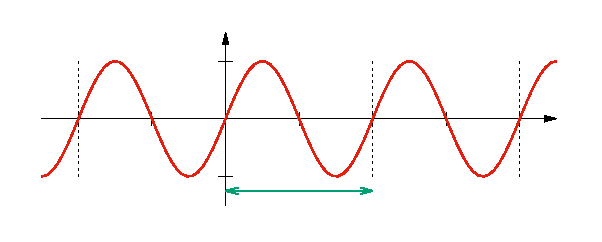
\includegraphics[width={273.60bp},height={100.70bp}]{figura_01_01}}%
    \gplfronttext
  \end{picture}%
\endgroup

    \caption{Función periódica}\label{figura_01}
\end{figure}

Una función periódica es aquella cuya gráfica se repite infinitas veces, cada
cierto intervalo (\textbf{Figura~\ref{figura_01}}).

El menor intervalo de repetición se llama \emph{periodo} ($T$).

Matemáticamente una función periódica es aquella que verifica:
\begin{equation}
    f(t)=f(t+nT);n\in\mathbb{Z}
\label{funcion_periodica}
\end{equation}

Donde $T$ es el periodo (la menor constante que verifica la igualdad).

\section{Propiedades de la funciones periódicas}
Si $f(t)=f(t+nT)$:
\subsection*{Propiedad 1}
\begin{equation}
    \int_a^b\,f(t)\,dt=\int_{a+nT}^{b+nT}f(t)\,dt\quad\,n\in\mathbb{Z}
\label{propiedad1}
\end{equation}

\underline{Prueba}:
\begin{equation*}
    \int_a^b\,f(t)\,dt=\int_{a}^{b}\,f(t+nT)\,dt
\end{equation*}

Cambiando la variable:
\begin{equation*}
    \tau=t+nT
\end{equation*}
\begin{equation*}
    d\tau=dt
\end{equation*}
\begin{equation*}
\begin{split}
    \int_a^b\,f(t)\,dt
        &=\int_{a+nT}^{b+nT}\,f(\tau)\,d\tau\\
        &=\int_{a+nT}^{b+nT}\,f(t)\,dt
\end{split}
\end{equation*}

Puede verse gráficamente en la \textbf{Figura~\ref{figura_02}}.
\begin{figure}[H]
    \centering
    % GNUPLOT: LaTeX picture with Postscript
\begingroup
  \makeatletter
  \providecommand\color[2][]{%
    \GenericError{(gnuplot) \space\space\space\@spaces}{%
      Package color not loaded in conjunction with
      terminal option `colourtext'%
    }{See the gnuplot documentation for explanation.%
    }{Either use 'blacktext' in gnuplot or load the package
      color.sty in LaTeX.}%
    \renewcommand\color[2][]{}%
  }%
  \providecommand\includegraphics[2][]{%
    \GenericError{(gnuplot) \space\space\space\@spaces}{%
      Package graphicx or graphics not loaded%
    }{See the gnuplot documentation for explanation.%
    }{The gnuplot epslatex terminal needs graphicx.sty or graphics.sty.}%
    \renewcommand\includegraphics[2][]{}%
  }%
  \providecommand\rotatebox[2]{#2}%
  \@ifundefined{ifGPcolor}{%
    \newif\ifGPcolor
    \GPcolorfalse
  }{}%
  \@ifundefined{ifGPblacktext}{%
    \newif\ifGPblacktext
    \GPblacktexttrue
  }{}%
  % define a \g@addto@macro without @ in the name:
  \let\gplgaddtomacro\g@addto@macro
  % define empty templates for all commands taking text:
  \gdef\gplbacktext{}%
  \gdef\gplfronttext{}%
  \makeatother
  \ifGPblacktext
    % no textcolor at all
    \def\colorrgb#1{}%
    \def\colorgray#1{}%
  \else
    % gray or color?
    \ifGPcolor
      \def\colorrgb#1{\color[rgb]{#1}}%
      \def\colorgray#1{\color[gray]{#1}}%
      \expandafter\def\csname LTw\endcsname{\color{white}}%
      \expandafter\def\csname LTb\endcsname{\color{black}}%
      \expandafter\def\csname LTa\endcsname{\color{black}}%
      \expandafter\def\csname LT0\endcsname{\color[rgb]{1,0,0}}%
      \expandafter\def\csname LT1\endcsname{\color[rgb]{0,1,0}}%
      \expandafter\def\csname LT2\endcsname{\color[rgb]{0,0,1}}%
      \expandafter\def\csname LT3\endcsname{\color[rgb]{1,0,1}}%
      \expandafter\def\csname LT4\endcsname{\color[rgb]{0,1,1}}%
      \expandafter\def\csname LT5\endcsname{\color[rgb]{1,1,0}}%
      \expandafter\def\csname LT6\endcsname{\color[rgb]{0,0,0}}%
      \expandafter\def\csname LT7\endcsname{\color[rgb]{1,0.3,0}}%
      \expandafter\def\csname LT8\endcsname{\color[rgb]{0.5,0.5,0.5}}%
    \else
      % gray
      \def\colorrgb#1{\color{black}}%
      \def\colorgray#1{\color[gray]{#1}}%
      \expandafter\def\csname LTw\endcsname{\color{white}}%
      \expandafter\def\csname LTb\endcsname{\color{black}}%
      \expandafter\def\csname LTa\endcsname{\color{black}}%
      \expandafter\def\csname LT0\endcsname{\color{black}}%
      \expandafter\def\csname LT1\endcsname{\color{black}}%
      \expandafter\def\csname LT2\endcsname{\color{black}}%
      \expandafter\def\csname LT3\endcsname{\color{black}}%
      \expandafter\def\csname LT4\endcsname{\color{black}}%
      \expandafter\def\csname LT5\endcsname{\color{black}}%
      \expandafter\def\csname LT6\endcsname{\color{black}}%
      \expandafter\def\csname LT7\endcsname{\color{black}}%
      \expandafter\def\csname LT8\endcsname{\color{black}}%
    \fi
  \fi
    \setlength{\unitlength}{0.0500bp}%
    \ifx\gptboxheight\undefined%
      \newlength{\gptboxheight}%
      \newlength{\gptboxwidth}%
      \newsavebox{\gptboxtext}%
    \fi%
    \setlength{\fboxrule}{0.5pt}%
    \setlength{\fboxsep}{1pt}%
    \definecolor{tbcol}{rgb}{1,1,1}%
\begin{picture}(6336.00,2590.00)%
    \gplgaddtomacro\gplbacktext{%
      \csname LTb\endcsname%%
      \put(1233,416){\makebox(0,0)[r]{\strut{}}}%
      \put(1233,863){\makebox(0,0)[r]{\strut{}}}%
      \put(1233,1311){\makebox(0,0)[r]{\strut{}}}%
      \put(1233,1758){\makebox(0,0)[r]{\strut{}}}%
      \put(1233,2205){\makebox(0,0)[r]{\strut{}}}%
      \put(603,640){\makebox(0,0){\strut{}}}%
      \put(1329,640){\makebox(0,0){\strut{}}}%
      \put(2055,640){\makebox(0,0){\strut{}}}%
      \put(2781,640){\makebox(0,0){\strut{}}}%
      \put(3506,640){\makebox(0,0){\strut{}}}%
      \put(4232,640){\makebox(0,0){\strut{}}}%
      \put(4958,640){\makebox(0,0){\strut{}}}%
      \put(5684,640){\makebox(0,0){\strut{}}}%
      \csname LTb\endcsname%%
      \put(6228,863){\makebox(0,0)[l]{\strut{}$t$}}%
      \put(1502,2429){\makebox(0,0)[l]{\strut{}$f(t)$}}%
      \put(2020,662){\makebox(0,0)[l]{\strut{}$a$}}%
      \put(2746,662){\makebox(0,0)[l]{\strut{}$b$}}%
      \put(3955,662){\makebox(0,0)[l]{\strut{}$a+T$}}%
      \put(4704,662){\makebox(0,0)[l]{\strut{}$b+T$}}%
      \put(1766,1982){\makebox(0,0)[l]{\strut{}$\int_a^b f(t) dt$}}%
      \put(3943,2295){\makebox(0,0)[l]{\strut{}$\int_{a+T}^{b+T} f(t+T) dt$}}%
    }%
    \gplgaddtomacro\gplfronttext{%
    }%
    \gplgaddtomacro\gplbacktext{%
      \csname LTb\endcsname%%
      \put(1233,416){\makebox(0,0)[r]{\strut{}}}%
      \put(1233,863){\makebox(0,0)[r]{\strut{}}}%
      \put(1233,1311){\makebox(0,0)[r]{\strut{}}}%
      \put(1233,1758){\makebox(0,0)[r]{\strut{}}}%
      \put(1233,2205){\makebox(0,0)[r]{\strut{}}}%
      \put(603,640){\makebox(0,0){\strut{}}}%
      \put(1329,640){\makebox(0,0){\strut{}}}%
      \put(2055,640){\makebox(0,0){\strut{}}}%
      \put(2781,640){\makebox(0,0){\strut{}}}%
      \put(3506,640){\makebox(0,0){\strut{}}}%
      \put(4232,640){\makebox(0,0){\strut{}}}%
      \put(4958,640){\makebox(0,0){\strut{}}}%
      \put(5684,640){\makebox(0,0){\strut{}}}%
      \csname LTb\endcsname%%
      \put(6228,863){\makebox(0,0)[l]{\strut{}$t$}}%
      \put(1502,2429){\makebox(0,0)[l]{\strut{}$f(t)$}}%
      \put(2020,662){\makebox(0,0)[l]{\strut{}$a$}}%
      \put(2746,662){\makebox(0,0)[l]{\strut{}$b$}}%
      \put(3955,662){\makebox(0,0)[l]{\strut{}$a+T$}}%
      \put(4704,662){\makebox(0,0)[l]{\strut{}$b+T$}}%
      \put(1766,1982){\makebox(0,0)[l]{\strut{}$\int_a^b f(t) dt$}}%
      \put(3943,2295){\makebox(0,0)[l]{\strut{}$\int_{a+T}^{b+T} f(t+T) dt$}}%
    }%
    \gplgaddtomacro\gplfronttext{%
    }%
    \gplgaddtomacro\gplbacktext{%
      \csname LTb\endcsname%%
      \put(1233,416){\makebox(0,0)[r]{\strut{}}}%
      \put(1233,863){\makebox(0,0)[r]{\strut{}}}%
      \put(1233,1311){\makebox(0,0)[r]{\strut{}}}%
      \put(1233,1758){\makebox(0,0)[r]{\strut{}}}%
      \put(1233,2205){\makebox(0,0)[r]{\strut{}}}%
      \put(603,640){\makebox(0,0){\strut{}}}%
      \put(1329,640){\makebox(0,0){\strut{}}}%
      \put(2055,640){\makebox(0,0){\strut{}}}%
      \put(2781,640){\makebox(0,0){\strut{}}}%
      \put(3506,640){\makebox(0,0){\strut{}}}%
      \put(4232,640){\makebox(0,0){\strut{}}}%
      \put(4958,640){\makebox(0,0){\strut{}}}%
      \put(5684,640){\makebox(0,0){\strut{}}}%
      \csname LTb\endcsname%%
      \put(6228,863){\makebox(0,0)[l]{\strut{}$t$}}%
      \put(1502,2429){\makebox(0,0)[l]{\strut{}$f(t)$}}%
      \put(2020,662){\makebox(0,0)[l]{\strut{}$a$}}%
      \put(2746,662){\makebox(0,0)[l]{\strut{}$b$}}%
      \put(3955,662){\makebox(0,0)[l]{\strut{}$a+T$}}%
      \put(4704,662){\makebox(0,0)[l]{\strut{}$b+T$}}%
      \put(1766,1982){\makebox(0,0)[l]{\strut{}$\int_a^b f(t) dt$}}%
      \put(3943,2295){\makebox(0,0)[l]{\strut{}$\int_{a+T}^{b+T} f(t+T) dt$}}%
    }%
    \gplgaddtomacro\gplfronttext{%
    }%
    \gplgaddtomacro\gplbacktext{%
      \csname LTb\endcsname%%
      \put(1233,416){\makebox(0,0)[r]{\strut{}}}%
      \put(1233,863){\makebox(0,0)[r]{\strut{}}}%
      \put(1233,1311){\makebox(0,0)[r]{\strut{}}}%
      \put(1233,1758){\makebox(0,0)[r]{\strut{}}}%
      \put(1233,2205){\makebox(0,0)[r]{\strut{}}}%
      \put(603,640){\makebox(0,0){\strut{}}}%
      \put(1329,640){\makebox(0,0){\strut{}}}%
      \put(2055,640){\makebox(0,0){\strut{}}}%
      \put(2781,640){\makebox(0,0){\strut{}}}%
      \put(3506,640){\makebox(0,0){\strut{}}}%
      \put(4232,640){\makebox(0,0){\strut{}}}%
      \put(4958,640){\makebox(0,0){\strut{}}}%
      \put(5684,640){\makebox(0,0){\strut{}}}%
      \csname LTb\endcsname%%
      \put(6228,863){\makebox(0,0)[l]{\strut{}$t$}}%
      \put(1502,2429){\makebox(0,0)[l]{\strut{}$f(t)$}}%
      \put(2020,662){\makebox(0,0)[l]{\strut{}$a$}}%
      \put(2746,662){\makebox(0,0)[l]{\strut{}$b$}}%
      \put(3955,662){\makebox(0,0)[l]{\strut{}$a+T$}}%
      \put(4704,662){\makebox(0,0)[l]{\strut{}$b+T$}}%
      \put(1766,1982){\makebox(0,0)[l]{\strut{}$\int_a^b f(t) dt$}}%
      \put(3943,2295){\makebox(0,0)[l]{\strut{}$\int_{a+T}^{b+T} f(t+T) dt$}}%
    }%
    \gplgaddtomacro\gplfronttext{%
    }%
    \gplgaddtomacro\gplbacktext{%
      \csname LTb\endcsname%%
      \put(1233,416){\makebox(0,0)[r]{\strut{}}}%
      \put(1233,863){\makebox(0,0)[r]{\strut{}}}%
      \put(1233,1311){\makebox(0,0)[r]{\strut{}}}%
      \put(1233,1758){\makebox(0,0)[r]{\strut{}}}%
      \put(1233,2205){\makebox(0,0)[r]{\strut{}}}%
      \put(603,640){\makebox(0,0){\strut{}}}%
      \put(1329,640){\makebox(0,0){\strut{}}}%
      \put(2055,640){\makebox(0,0){\strut{}}}%
      \put(2781,640){\makebox(0,0){\strut{}}}%
      \put(3506,640){\makebox(0,0){\strut{}}}%
      \put(4232,640){\makebox(0,0){\strut{}}}%
      \put(4958,640){\makebox(0,0){\strut{}}}%
      \put(5684,640){\makebox(0,0){\strut{}}}%
      \csname LTb\endcsname%%
      \put(6228,863){\makebox(0,0)[l]{\strut{}$t$}}%
      \put(1502,2429){\makebox(0,0)[l]{\strut{}$f(t)$}}%
      \put(2020,662){\makebox(0,0)[l]{\strut{}$a$}}%
      \put(2746,662){\makebox(0,0)[l]{\strut{}$b$}}%
      \put(3955,662){\makebox(0,0)[l]{\strut{}$a+T$}}%
      \put(4704,662){\makebox(0,0)[l]{\strut{}$b+T$}}%
      \put(1766,1982){\makebox(0,0)[l]{\strut{}$\int_a^b f(t) dt$}}%
      \put(3943,2295){\makebox(0,0)[l]{\strut{}$\int_{a+T}^{b+T} f(t+T) dt$}}%
    }%
    \gplgaddtomacro\gplfronttext{%
    }%
    \gplgaddtomacro\gplbacktext{%
      \csname LTb\endcsname%%
      \put(1233,416){\makebox(0,0)[r]{\strut{}}}%
      \put(1233,863){\makebox(0,0)[r]{\strut{}}}%
      \put(1233,1311){\makebox(0,0)[r]{\strut{}}}%
      \put(1233,1758){\makebox(0,0)[r]{\strut{}}}%
      \put(1233,2205){\makebox(0,0)[r]{\strut{}}}%
      \put(603,640){\makebox(0,0){\strut{}}}%
      \put(1329,640){\makebox(0,0){\strut{}}}%
      \put(2055,640){\makebox(0,0){\strut{}}}%
      \put(2781,640){\makebox(0,0){\strut{}}}%
      \put(3506,640){\makebox(0,0){\strut{}}}%
      \put(4232,640){\makebox(0,0){\strut{}}}%
      \put(4958,640){\makebox(0,0){\strut{}}}%
      \put(5684,640){\makebox(0,0){\strut{}}}%
      \csname LTb\endcsname%%
      \put(6228,863){\makebox(0,0)[l]{\strut{}$t$}}%
      \put(1502,2429){\makebox(0,0)[l]{\strut{}$f(t)$}}%
      \put(2020,662){\makebox(0,0)[l]{\strut{}$a$}}%
      \put(2746,662){\makebox(0,0)[l]{\strut{}$b$}}%
      \put(3955,662){\makebox(0,0)[l]{\strut{}$a+T$}}%
      \put(4704,662){\makebox(0,0)[l]{\strut{}$b+T$}}%
      \put(1766,1982){\makebox(0,0)[l]{\strut{}$\int_a^b f(t) dt$}}%
      \put(3943,2295){\makebox(0,0)[l]{\strut{}$\int_{a+T}^{b+T} f(t+T) dt$}}%
    }%
    \gplgaddtomacro\gplfronttext{%
    }%
    \gplbacktext
    \put(0,0){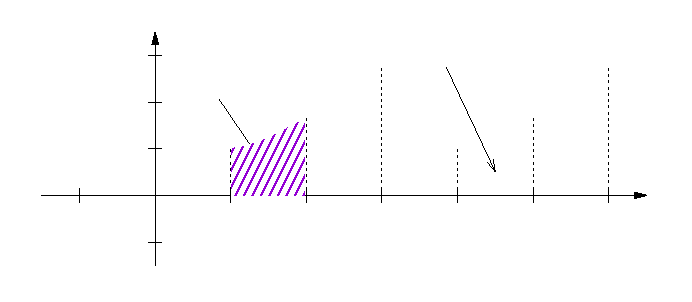
\includegraphics[width={316.80bp},height={129.50bp}]{figura_01_02}}%
    \gplfronttext
  \end{picture}%
\endgroup

    \caption{Demostración gráfica}\label{figura_02}
\end{figure}

\subsection*{Propiedad 2}
\begin{equation}
    \int_{a-T/2}^{a+T/2}f(t)\,dt=\int_{-T/2}^{T/2}f(t)\,dt
\label{propiedad2}
\end{equation}

\underline{Prueba}:
\begin{equation*}
\begin{split}
    \int_{a-T/2}^{a+T/2}f(t)\,dt
        &=\int_{a-T/2}^{T/2}f(t)\,dt+\int_{T/2}^{a+T/2}f(t)\,dt\\
        &=\int_{a-T/2}^{T/2}f(t)\,dt+\int_{T/2-T}^{a+T/2-T}f(t)\,dt\\
        &=\int_{a-T/2}^{T/2}f(t)\,dt+\int_{-T/2}^{a-T/2}f(t)\,dt\\
        &=\int_{-T/2}^{T/2}f(t)\,dt
\end{split}
\end{equation*}

Puede verse gráficamente en la \textbf{Figura~\ref{figura_03}}.
\begin{figure}[H]
    \centering
    % GNUPLOT: LaTeX picture with Postscript
\begingroup
  \makeatletter
  \providecommand\color[2][]{%
    \GenericError{(gnuplot) \space\space\space\@spaces}{%
      Package color not loaded in conjunction with
      terminal option `colourtext'%
    }{See the gnuplot documentation for explanation.%
    }{Either use 'blacktext' in gnuplot or load the package
      color.sty in LaTeX.}%
    \renewcommand\color[2][]{}%
  }%
  \providecommand\includegraphics[2][]{%
    \GenericError{(gnuplot) \space\space\space\@spaces}{%
      Package graphicx or graphics not loaded%
    }{See the gnuplot documentation for explanation.%
    }{The gnuplot epslatex terminal needs graphicx.sty or graphics.sty.}%
    \renewcommand\includegraphics[2][]{}%
  }%
  \providecommand\rotatebox[2]{#2}%
  \@ifundefined{ifGPcolor}{%
    \newif\ifGPcolor
    \GPcolorfalse
  }{}%
  \@ifundefined{ifGPblacktext}{%
    \newif\ifGPblacktext
    \GPblacktexttrue
  }{}%
  % define a \g@addto@macro without @ in the name:
  \let\gplgaddtomacro\g@addto@macro
  % define empty templates for all commands taking text:
  \gdef\gplbacktext{}%
  \gdef\gplfronttext{}%
  \makeatother
  \ifGPblacktext
    % no textcolor at all
    \def\colorrgb#1{}%
    \def\colorgray#1{}%
  \else
    % gray or color?
    \ifGPcolor
      \def\colorrgb#1{\color[rgb]{#1}}%
      \def\colorgray#1{\color[gray]{#1}}%
      \expandafter\def\csname LTw\endcsname{\color{white}}%
      \expandafter\def\csname LTb\endcsname{\color{black}}%
      \expandafter\def\csname LTa\endcsname{\color{black}}%
      \expandafter\def\csname LT0\endcsname{\color[rgb]{1,0,0}}%
      \expandafter\def\csname LT1\endcsname{\color[rgb]{0,1,0}}%
      \expandafter\def\csname LT2\endcsname{\color[rgb]{0,0,1}}%
      \expandafter\def\csname LT3\endcsname{\color[rgb]{1,0,1}}%
      \expandafter\def\csname LT4\endcsname{\color[rgb]{0,1,1}}%
      \expandafter\def\csname LT5\endcsname{\color[rgb]{1,1,0}}%
      \expandafter\def\csname LT6\endcsname{\color[rgb]{0,0,0}}%
      \expandafter\def\csname LT7\endcsname{\color[rgb]{1,0.3,0}}%
      \expandafter\def\csname LT8\endcsname{\color[rgb]{0.5,0.5,0.5}}%
    \else
      % gray
      \def\colorrgb#1{\color{black}}%
      \def\colorgray#1{\color[gray]{#1}}%
      \expandafter\def\csname LTw\endcsname{\color{white}}%
      \expandafter\def\csname LTb\endcsname{\color{black}}%
      \expandafter\def\csname LTa\endcsname{\color{black}}%
      \expandafter\def\csname LT0\endcsname{\color{black}}%
      \expandafter\def\csname LT1\endcsname{\color{black}}%
      \expandafter\def\csname LT2\endcsname{\color{black}}%
      \expandafter\def\csname LT3\endcsname{\color{black}}%
      \expandafter\def\csname LT4\endcsname{\color{black}}%
      \expandafter\def\csname LT5\endcsname{\color{black}}%
      \expandafter\def\csname LT6\endcsname{\color{black}}%
      \expandafter\def\csname LT7\endcsname{\color{black}}%
      \expandafter\def\csname LT8\endcsname{\color{black}}%
    \fi
  \fi
    \setlength{\unitlength}{0.0500bp}%
    \ifx\gptboxheight\undefined%
      \newlength{\gptboxheight}%
      \newlength{\gptboxwidth}%
      \newsavebox{\gptboxtext}%
    \fi%
    \setlength{\fboxrule}{0.5pt}%
    \setlength{\fboxsep}{1pt}%
    \definecolor{tbcol}{rgb}{1,1,1}%
\begin{picture}(6336.00,2590.00)%
    \gplgaddtomacro\gplbacktext{%
      \csname LTb\endcsname%%
      \put(1757,416){\makebox(0,0)[r]{\strut{}}}%
      \put(1757,863){\makebox(0,0)[r]{\strut{}}}%
      \put(1757,1311){\makebox(0,0)[r]{\strut{}}}%
      \put(1757,1758){\makebox(0,0)[r]{\strut{}}}%
      \put(1757,2205){\makebox(0,0)[r]{\strut{}}}%
      \put(563,640){\makebox(0,0){\strut{}}}%
      \put(1208,640){\makebox(0,0){\strut{}}}%
      \put(1853,640){\makebox(0,0){\strut{}}}%
      \put(2498,640){\makebox(0,0){\strut{}}}%
      \put(3143,640){\makebox(0,0){\strut{}}}%
      \put(3789,640){\makebox(0,0){\strut{}}}%
      \put(4434,640){\makebox(0,0){\strut{}}}%
      \put(5079,640){\makebox(0,0){\strut{}}}%
      \put(5724,640){\makebox(0,0){\strut{}}}%
      \csname LTb\endcsname%%
      \put(6208,863){\makebox(0,0)[l]{\strut{}$t$}}%
      \put(2007,2429){\makebox(0,0)[l]{\strut{}$f(t)$}}%
      \put(631,662){\makebox(0,0)[l]{\strut{}$-\frac{T}{2}$}}%
      \put(2728,662){\makebox(0,0)[l]{\strut{}$\frac{T}{2}$}}%
      \put(3203,662){\makebox(0,0)[l]{\strut{}$a-\frac{T}{2}$}}%
      \put(4383,662){\makebox(0,0)[l]{\strut{}$a$}}%
      \put(5201,662){\makebox(0,0)[l]{\strut{}$a+\frac{T}{2}$}}%
      \put(306,2026){\makebox(0,0)[l]{\strut{}$\int_{-\frac{T}{2}}^{\frac{T}{2}} f(t) dt$}}%
      \put(4177,2295){\makebox(0,0)[l]{\strut{}$\int_{a-\frac{T}{2}}^{a+\frac{T}{2}} f(t) dt$}}%
    }%
    \gplgaddtomacro\gplfronttext{%
    }%
    \gplgaddtomacro\gplbacktext{%
      \csname LTb\endcsname%%
      \put(1757,416){\makebox(0,0)[r]{\strut{}}}%
      \put(1757,863){\makebox(0,0)[r]{\strut{}}}%
      \put(1757,1311){\makebox(0,0)[r]{\strut{}}}%
      \put(1757,1758){\makebox(0,0)[r]{\strut{}}}%
      \put(1757,2205){\makebox(0,0)[r]{\strut{}}}%
      \put(563,640){\makebox(0,0){\strut{}}}%
      \put(1208,640){\makebox(0,0){\strut{}}}%
      \put(1853,640){\makebox(0,0){\strut{}}}%
      \put(2498,640){\makebox(0,0){\strut{}}}%
      \put(3143,640){\makebox(0,0){\strut{}}}%
      \put(3789,640){\makebox(0,0){\strut{}}}%
      \put(4434,640){\makebox(0,0){\strut{}}}%
      \put(5079,640){\makebox(0,0){\strut{}}}%
      \put(5724,640){\makebox(0,0){\strut{}}}%
      \csname LTb\endcsname%%
      \put(6208,863){\makebox(0,0)[l]{\strut{}$t$}}%
      \put(2007,2429){\makebox(0,0)[l]{\strut{}$f(t)$}}%
      \put(631,662){\makebox(0,0)[l]{\strut{}$-\frac{T}{2}$}}%
      \put(2728,662){\makebox(0,0)[l]{\strut{}$\frac{T}{2}$}}%
      \put(3203,662){\makebox(0,0)[l]{\strut{}$a-\frac{T}{2}$}}%
      \put(4383,662){\makebox(0,0)[l]{\strut{}$a$}}%
      \put(5201,662){\makebox(0,0)[l]{\strut{}$a+\frac{T}{2}$}}%
      \put(306,2026){\makebox(0,0)[l]{\strut{}$\int_{-\frac{T}{2}}^{\frac{T}{2}} f(t) dt$}}%
      \put(4177,2295){\makebox(0,0)[l]{\strut{}$\int_{a-\frac{T}{2}}^{a+\frac{T}{2}} f(t) dt$}}%
    }%
    \gplgaddtomacro\gplfronttext{%
    }%
    \gplgaddtomacro\gplbacktext{%
      \csname LTb\endcsname%%
      \put(1757,416){\makebox(0,0)[r]{\strut{}}}%
      \put(1757,863){\makebox(0,0)[r]{\strut{}}}%
      \put(1757,1311){\makebox(0,0)[r]{\strut{}}}%
      \put(1757,1758){\makebox(0,0)[r]{\strut{}}}%
      \put(1757,2205){\makebox(0,0)[r]{\strut{}}}%
      \put(563,640){\makebox(0,0){\strut{}}}%
      \put(1208,640){\makebox(0,0){\strut{}}}%
      \put(1853,640){\makebox(0,0){\strut{}}}%
      \put(2498,640){\makebox(0,0){\strut{}}}%
      \put(3143,640){\makebox(0,0){\strut{}}}%
      \put(3789,640){\makebox(0,0){\strut{}}}%
      \put(4434,640){\makebox(0,0){\strut{}}}%
      \put(5079,640){\makebox(0,0){\strut{}}}%
      \put(5724,640){\makebox(0,0){\strut{}}}%
      \csname LTb\endcsname%%
      \put(6208,863){\makebox(0,0)[l]{\strut{}$t$}}%
      \put(2007,2429){\makebox(0,0)[l]{\strut{}$f(t)$}}%
      \put(631,662){\makebox(0,0)[l]{\strut{}$-\frac{T}{2}$}}%
      \put(2728,662){\makebox(0,0)[l]{\strut{}$\frac{T}{2}$}}%
      \put(3203,662){\makebox(0,0)[l]{\strut{}$a-\frac{T}{2}$}}%
      \put(4383,662){\makebox(0,0)[l]{\strut{}$a$}}%
      \put(5201,662){\makebox(0,0)[l]{\strut{}$a+\frac{T}{2}$}}%
      \put(306,2026){\makebox(0,0)[l]{\strut{}$\int_{-\frac{T}{2}}^{\frac{T}{2}} f(t) dt$}}%
      \put(4177,2295){\makebox(0,0)[l]{\strut{}$\int_{a-\frac{T}{2}}^{a+\frac{T}{2}} f(t) dt$}}%
    }%
    \gplgaddtomacro\gplfronttext{%
    }%
    \gplgaddtomacro\gplbacktext{%
      \csname LTb\endcsname%%
      \put(1757,416){\makebox(0,0)[r]{\strut{}}}%
      \put(1757,863){\makebox(0,0)[r]{\strut{}}}%
      \put(1757,1311){\makebox(0,0)[r]{\strut{}}}%
      \put(1757,1758){\makebox(0,0)[r]{\strut{}}}%
      \put(1757,2205){\makebox(0,0)[r]{\strut{}}}%
      \put(563,640){\makebox(0,0){\strut{}}}%
      \put(1208,640){\makebox(0,0){\strut{}}}%
      \put(1853,640){\makebox(0,0){\strut{}}}%
      \put(2498,640){\makebox(0,0){\strut{}}}%
      \put(3143,640){\makebox(0,0){\strut{}}}%
      \put(3789,640){\makebox(0,0){\strut{}}}%
      \put(4434,640){\makebox(0,0){\strut{}}}%
      \put(5079,640){\makebox(0,0){\strut{}}}%
      \put(5724,640){\makebox(0,0){\strut{}}}%
      \csname LTb\endcsname%%
      \put(6208,863){\makebox(0,0)[l]{\strut{}$t$}}%
      \put(2007,2429){\makebox(0,0)[l]{\strut{}$f(t)$}}%
      \put(631,662){\makebox(0,0)[l]{\strut{}$-\frac{T}{2}$}}%
      \put(2728,662){\makebox(0,0)[l]{\strut{}$\frac{T}{2}$}}%
      \put(3203,662){\makebox(0,0)[l]{\strut{}$a-\frac{T}{2}$}}%
      \put(4383,662){\makebox(0,0)[l]{\strut{}$a$}}%
      \put(5201,662){\makebox(0,0)[l]{\strut{}$a+\frac{T}{2}$}}%
      \put(306,2026){\makebox(0,0)[l]{\strut{}$\int_{-\frac{T}{2}}^{\frac{T}{2}} f(t) dt$}}%
      \put(4177,2295){\makebox(0,0)[l]{\strut{}$\int_{a-\frac{T}{2}}^{a+\frac{T}{2}} f(t) dt$}}%
    }%
    \gplgaddtomacro\gplfronttext{%
    }%
    \gplgaddtomacro\gplbacktext{%
      \csname LTb\endcsname%%
      \put(1757,416){\makebox(0,0)[r]{\strut{}}}%
      \put(1757,863){\makebox(0,0)[r]{\strut{}}}%
      \put(1757,1311){\makebox(0,0)[r]{\strut{}}}%
      \put(1757,1758){\makebox(0,0)[r]{\strut{}}}%
      \put(1757,2205){\makebox(0,0)[r]{\strut{}}}%
      \put(563,640){\makebox(0,0){\strut{}}}%
      \put(1208,640){\makebox(0,0){\strut{}}}%
      \put(1853,640){\makebox(0,0){\strut{}}}%
      \put(2498,640){\makebox(0,0){\strut{}}}%
      \put(3143,640){\makebox(0,0){\strut{}}}%
      \put(3789,640){\makebox(0,0){\strut{}}}%
      \put(4434,640){\makebox(0,0){\strut{}}}%
      \put(5079,640){\makebox(0,0){\strut{}}}%
      \put(5724,640){\makebox(0,0){\strut{}}}%
      \csname LTb\endcsname%%
      \put(6208,863){\makebox(0,0)[l]{\strut{}$t$}}%
      \put(2007,2429){\makebox(0,0)[l]{\strut{}$f(t)$}}%
      \put(631,662){\makebox(0,0)[l]{\strut{}$-\frac{T}{2}$}}%
      \put(2728,662){\makebox(0,0)[l]{\strut{}$\frac{T}{2}$}}%
      \put(3203,662){\makebox(0,0)[l]{\strut{}$a-\frac{T}{2}$}}%
      \put(4383,662){\makebox(0,0)[l]{\strut{}$a$}}%
      \put(5201,662){\makebox(0,0)[l]{\strut{}$a+\frac{T}{2}$}}%
      \put(306,2026){\makebox(0,0)[l]{\strut{}$\int_{-\frac{T}{2}}^{\frac{T}{2}} f(t) dt$}}%
      \put(4177,2295){\makebox(0,0)[l]{\strut{}$\int_{a-\frac{T}{2}}^{a+\frac{T}{2}} f(t) dt$}}%
    }%
    \gplgaddtomacro\gplfronttext{%
    }%
    \gplgaddtomacro\gplbacktext{%
      \csname LTb\endcsname%%
      \put(1757,416){\makebox(0,0)[r]{\strut{}}}%
      \put(1757,863){\makebox(0,0)[r]{\strut{}}}%
      \put(1757,1311){\makebox(0,0)[r]{\strut{}}}%
      \put(1757,1758){\makebox(0,0)[r]{\strut{}}}%
      \put(1757,2205){\makebox(0,0)[r]{\strut{}}}%
      \put(563,640){\makebox(0,0){\strut{}}}%
      \put(1208,640){\makebox(0,0){\strut{}}}%
      \put(1853,640){\makebox(0,0){\strut{}}}%
      \put(2498,640){\makebox(0,0){\strut{}}}%
      \put(3143,640){\makebox(0,0){\strut{}}}%
      \put(3789,640){\makebox(0,0){\strut{}}}%
      \put(4434,640){\makebox(0,0){\strut{}}}%
      \put(5079,640){\makebox(0,0){\strut{}}}%
      \put(5724,640){\makebox(0,0){\strut{}}}%
      \csname LTb\endcsname%%
      \put(6208,863){\makebox(0,0)[l]{\strut{}$t$}}%
      \put(2007,2429){\makebox(0,0)[l]{\strut{}$f(t)$}}%
      \put(631,662){\makebox(0,0)[l]{\strut{}$-\frac{T}{2}$}}%
      \put(2728,662){\makebox(0,0)[l]{\strut{}$\frac{T}{2}$}}%
      \put(3203,662){\makebox(0,0)[l]{\strut{}$a-\frac{T}{2}$}}%
      \put(4383,662){\makebox(0,0)[l]{\strut{}$a$}}%
      \put(5201,662){\makebox(0,0)[l]{\strut{}$a+\frac{T}{2}$}}%
      \put(306,2026){\makebox(0,0)[l]{\strut{}$\int_{-\frac{T}{2}}^{\frac{T}{2}} f(t) dt$}}%
      \put(4177,2295){\makebox(0,0)[l]{\strut{}$\int_{a-\frac{T}{2}}^{a+\frac{T}{2}} f(t) dt$}}%
    }%
    \gplgaddtomacro\gplfronttext{%
    }%
    \gplgaddtomacro\gplbacktext{%
      \csname LTb\endcsname%%
      \put(1757,416){\makebox(0,0)[r]{\strut{}}}%
      \put(1757,863){\makebox(0,0)[r]{\strut{}}}%
      \put(1757,1311){\makebox(0,0)[r]{\strut{}}}%
      \put(1757,1758){\makebox(0,0)[r]{\strut{}}}%
      \put(1757,2205){\makebox(0,0)[r]{\strut{}}}%
      \put(563,640){\makebox(0,0){\strut{}}}%
      \put(1208,640){\makebox(0,0){\strut{}}}%
      \put(1853,640){\makebox(0,0){\strut{}}}%
      \put(2498,640){\makebox(0,0){\strut{}}}%
      \put(3143,640){\makebox(0,0){\strut{}}}%
      \put(3789,640){\makebox(0,0){\strut{}}}%
      \put(4434,640){\makebox(0,0){\strut{}}}%
      \put(5079,640){\makebox(0,0){\strut{}}}%
      \put(5724,640){\makebox(0,0){\strut{}}}%
      \csname LTb\endcsname%%
      \put(6208,863){\makebox(0,0)[l]{\strut{}$t$}}%
      \put(2007,2429){\makebox(0,0)[l]{\strut{}$f(t)$}}%
      \put(631,662){\makebox(0,0)[l]{\strut{}$-\frac{T}{2}$}}%
      \put(2728,662){\makebox(0,0)[l]{\strut{}$\frac{T}{2}$}}%
      \put(3203,662){\makebox(0,0)[l]{\strut{}$a-\frac{T}{2}$}}%
      \put(4383,662){\makebox(0,0)[l]{\strut{}$a$}}%
      \put(5201,662){\makebox(0,0)[l]{\strut{}$a+\frac{T}{2}$}}%
      \put(306,2026){\makebox(0,0)[l]{\strut{}$\int_{-\frac{T}{2}}^{\frac{T}{2}} f(t) dt$}}%
      \put(4177,2295){\makebox(0,0)[l]{\strut{}$\int_{a-\frac{T}{2}}^{a+\frac{T}{2}} f(t) dt$}}%
    }%
    \gplgaddtomacro\gplfronttext{%
    }%
    \gplgaddtomacro\gplbacktext{%
      \csname LTb\endcsname%%
      \put(1757,416){\makebox(0,0)[r]{\strut{}}}%
      \put(1757,863){\makebox(0,0)[r]{\strut{}}}%
      \put(1757,1311){\makebox(0,0)[r]{\strut{}}}%
      \put(1757,1758){\makebox(0,0)[r]{\strut{}}}%
      \put(1757,2205){\makebox(0,0)[r]{\strut{}}}%
      \put(563,640){\makebox(0,0){\strut{}}}%
      \put(1208,640){\makebox(0,0){\strut{}}}%
      \put(1853,640){\makebox(0,0){\strut{}}}%
      \put(2498,640){\makebox(0,0){\strut{}}}%
      \put(3143,640){\makebox(0,0){\strut{}}}%
      \put(3789,640){\makebox(0,0){\strut{}}}%
      \put(4434,640){\makebox(0,0){\strut{}}}%
      \put(5079,640){\makebox(0,0){\strut{}}}%
      \put(5724,640){\makebox(0,0){\strut{}}}%
      \csname LTb\endcsname%%
      \put(6208,863){\makebox(0,0)[l]{\strut{}$t$}}%
      \put(2007,2429){\makebox(0,0)[l]{\strut{}$f(t)$}}%
      \put(631,662){\makebox(0,0)[l]{\strut{}$-\frac{T}{2}$}}%
      \put(2728,662){\makebox(0,0)[l]{\strut{}$\frac{T}{2}$}}%
      \put(3203,662){\makebox(0,0)[l]{\strut{}$a-\frac{T}{2}$}}%
      \put(4383,662){\makebox(0,0)[l]{\strut{}$a$}}%
      \put(5201,662){\makebox(0,0)[l]{\strut{}$a+\frac{T}{2}$}}%
      \put(306,2026){\makebox(0,0)[l]{\strut{}$\int_{-\frac{T}{2}}^{\frac{T}{2}} f(t) dt$}}%
      \put(4177,2295){\makebox(0,0)[l]{\strut{}$\int_{a-\frac{T}{2}}^{a+\frac{T}{2}} f(t) dt$}}%
    }%
    \gplgaddtomacro\gplfronttext{%
    }%
    \gplbacktext
    \put(0,0){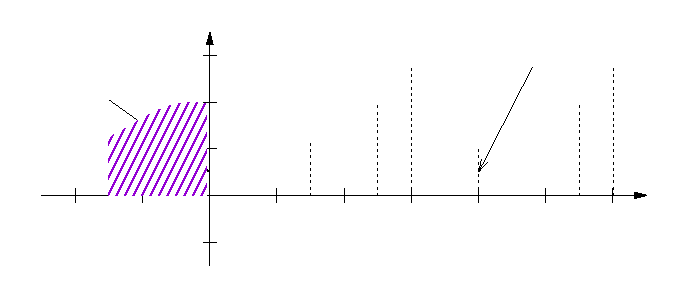
\includegraphics[width={316.80bp},height={129.50bp}]{figura_01_03}}%
    \gplfronttext
  \end{picture}%
\endgroup

    \caption{Demostración gráfica}\label{figura_03}
\end{figure}

\subsection*{Propiedad 3}
\begin{equation}
    \int_{0}^{T}f(t)\,dt=\int_{-T/2}^{T/2}f(t)\,dt
\label{propiedad3}
\end{equation}

\underline{Prueba}:

Si en la ecuación (\ref{propiedad2}) $a=T/2$:
\begin{equation*}
\begin{split}
    \int_{-T/2}^{T/2}f(t)\,dt
        &=\int_{a-T/2}^{a+T/2}f(t)\,dt\\
        &=\int_{T/2-T/2}^{T/2+T/2}f(t)\,dt\\
        &=\int_{0}^{T}f(t)\,dt
\end{split}
\end{equation*}

Puede verse gráficamente en la \textbf{Figura~\ref{figura_04}}.
\begin{figure}[H]
    \centering
    % GNUPLOT: LaTeX picture with Postscript
\begingroup
  \makeatletter
  \providecommand\color[2][]{%
    \GenericError{(gnuplot) \space\space\space\@spaces}{%
      Package color not loaded in conjunction with
      terminal option `colourtext'%
    }{See the gnuplot documentation for explanation.%
    }{Either use 'blacktext' in gnuplot or load the package
      color.sty in LaTeX.}%
    \renewcommand\color[2][]{}%
  }%
  \providecommand\includegraphics[2][]{%
    \GenericError{(gnuplot) \space\space\space\@spaces}{%
      Package graphicx or graphics not loaded%
    }{See the gnuplot documentation for explanation.%
    }{The gnuplot epslatex terminal needs graphicx.sty or graphics.sty.}%
    \renewcommand\includegraphics[2][]{}%
  }%
  \providecommand\rotatebox[2]{#2}%
  \@ifundefined{ifGPcolor}{%
    \newif\ifGPcolor
    \GPcolorfalse
  }{}%
  \@ifundefined{ifGPblacktext}{%
    \newif\ifGPblacktext
    \GPblacktexttrue
  }{}%
  % define a \g@addto@macro without @ in the name:
  \let\gplgaddtomacro\g@addto@macro
  % define empty templates for all commands taking text:
  \gdef\gplbacktext{}%
  \gdef\gplfronttext{}%
  \makeatother
  \ifGPblacktext
    % no textcolor at all
    \def\colorrgb#1{}%
    \def\colorgray#1{}%
  \else
    % gray or color?
    \ifGPcolor
      \def\colorrgb#1{\color[rgb]{#1}}%
      \def\colorgray#1{\color[gray]{#1}}%
      \expandafter\def\csname LTw\endcsname{\color{white}}%
      \expandafter\def\csname LTb\endcsname{\color{black}}%
      \expandafter\def\csname LTa\endcsname{\color{black}}%
      \expandafter\def\csname LT0\endcsname{\color[rgb]{1,0,0}}%
      \expandafter\def\csname LT1\endcsname{\color[rgb]{0,1,0}}%
      \expandafter\def\csname LT2\endcsname{\color[rgb]{0,0,1}}%
      \expandafter\def\csname LT3\endcsname{\color[rgb]{1,0,1}}%
      \expandafter\def\csname LT4\endcsname{\color[rgb]{0,1,1}}%
      \expandafter\def\csname LT5\endcsname{\color[rgb]{1,1,0}}%
      \expandafter\def\csname LT6\endcsname{\color[rgb]{0,0,0}}%
      \expandafter\def\csname LT7\endcsname{\color[rgb]{1,0.3,0}}%
      \expandafter\def\csname LT8\endcsname{\color[rgb]{0.5,0.5,0.5}}%
    \else
      % gray
      \def\colorrgb#1{\color{black}}%
      \def\colorgray#1{\color[gray]{#1}}%
      \expandafter\def\csname LTw\endcsname{\color{white}}%
      \expandafter\def\csname LTb\endcsname{\color{black}}%
      \expandafter\def\csname LTa\endcsname{\color{black}}%
      \expandafter\def\csname LT0\endcsname{\color{black}}%
      \expandafter\def\csname LT1\endcsname{\color{black}}%
      \expandafter\def\csname LT2\endcsname{\color{black}}%
      \expandafter\def\csname LT3\endcsname{\color{black}}%
      \expandafter\def\csname LT4\endcsname{\color{black}}%
      \expandafter\def\csname LT5\endcsname{\color{black}}%
      \expandafter\def\csname LT6\endcsname{\color{black}}%
      \expandafter\def\csname LT7\endcsname{\color{black}}%
      \expandafter\def\csname LT8\endcsname{\color{black}}%
    \fi
  \fi
    \setlength{\unitlength}{0.0500bp}%
    \ifx\gptboxheight\undefined%
      \newlength{\gptboxheight}%
      \newlength{\gptboxwidth}%
      \newsavebox{\gptboxtext}%
    \fi%
    \setlength{\fboxrule}{0.5pt}%
    \setlength{\fboxsep}{1pt}%
    \definecolor{tbcol}{rgb}{1,1,1}%
\begin{picture}(6336.00,2590.00)%
    \gplgaddtomacro\gplbacktext{%
      \csname LTb\endcsname%%
      \put(2356,455){\makebox(0,0)[r]{\strut{}}}%
      \put(2356,982){\makebox(0,0)[r]{\strut{}}}%
      \put(2356,1508){\makebox(0,0)[r]{\strut{}}}%
      \put(2356,2034){\makebox(0,0)[r]{\strut{}}}%
      \put(240,759){\makebox(0,0){\strut{}}}%
      \put(1346,759){\makebox(0,0){\strut{}}}%
      \put(2452,759){\makebox(0,0){\strut{}}}%
      \put(3558,759){\makebox(0,0){\strut{}}}%
      \put(4664,759){\makebox(0,0){\strut{}}}%
      \put(5770,759){\makebox(0,0){\strut{}}}%
      \csname LTb\endcsname%%
      \put(6324,982){\makebox(0,0)[l]{\strut{}$t$}}%
      \put(2628,2561){\makebox(0,0)[l]{\strut{}$f(t)$}}%
      \put(574,745){\makebox(0,0)[l]{\strut{}$-\frac{T}{2}$}}%
      \put(4059,745){\makebox(0,0)[l]{\strut{}$ \frac{T}{2}$}}%
      \put(5735,745){\makebox(0,0)[l]{\strut{}$T$}}%
      \put(265,2350){\makebox(0,0)[l]{\strut{}$\int_{-\frac{T}{2}}^{\frac{T}{2}} f(t) dt$}}%
      \put(3231,2350){\makebox(0,0)[l]{\strut{}$\int_{0}^{T} f(t) dt$}}%
    }%
    \gplgaddtomacro\gplfronttext{%
    }%
    \gplgaddtomacro\gplbacktext{%
      \csname LTb\endcsname%%
      \put(2356,455){\makebox(0,0)[r]{\strut{}}}%
      \put(2356,982){\makebox(0,0)[r]{\strut{}}}%
      \put(2356,1508){\makebox(0,0)[r]{\strut{}}}%
      \put(2356,2034){\makebox(0,0)[r]{\strut{}}}%
      \put(240,759){\makebox(0,0){\strut{}}}%
      \put(1346,759){\makebox(0,0){\strut{}}}%
      \put(2452,759){\makebox(0,0){\strut{}}}%
      \put(3558,759){\makebox(0,0){\strut{}}}%
      \put(4664,759){\makebox(0,0){\strut{}}}%
      \put(5770,759){\makebox(0,0){\strut{}}}%
      \csname LTb\endcsname%%
      \put(6324,982){\makebox(0,0)[l]{\strut{}$t$}}%
      \put(2628,2561){\makebox(0,0)[l]{\strut{}$f(t)$}}%
      \put(574,745){\makebox(0,0)[l]{\strut{}$-\frac{T}{2}$}}%
      \put(4059,745){\makebox(0,0)[l]{\strut{}$ \frac{T}{2}$}}%
      \put(5735,745){\makebox(0,0)[l]{\strut{}$T$}}%
      \put(265,2350){\makebox(0,0)[l]{\strut{}$\int_{-\frac{T}{2}}^{\frac{T}{2}} f(t) dt$}}%
      \put(3231,2350){\makebox(0,0)[l]{\strut{}$\int_{0}^{T} f(t) dt$}}%
    }%
    \gplgaddtomacro\gplfronttext{%
    }%
    \gplgaddtomacro\gplbacktext{%
      \csname LTb\endcsname%%
      \put(2356,455){\makebox(0,0)[r]{\strut{}}}%
      \put(2356,982){\makebox(0,0)[r]{\strut{}}}%
      \put(2356,1508){\makebox(0,0)[r]{\strut{}}}%
      \put(2356,2034){\makebox(0,0)[r]{\strut{}}}%
      \put(240,759){\makebox(0,0){\strut{}}}%
      \put(1346,759){\makebox(0,0){\strut{}}}%
      \put(2452,759){\makebox(0,0){\strut{}}}%
      \put(3558,759){\makebox(0,0){\strut{}}}%
      \put(4664,759){\makebox(0,0){\strut{}}}%
      \put(5770,759){\makebox(0,0){\strut{}}}%
      \csname LTb\endcsname%%
      \put(6324,982){\makebox(0,0)[l]{\strut{}$t$}}%
      \put(2628,2561){\makebox(0,0)[l]{\strut{}$f(t)$}}%
      \put(574,745){\makebox(0,0)[l]{\strut{}$-\frac{T}{2}$}}%
      \put(4059,745){\makebox(0,0)[l]{\strut{}$ \frac{T}{2}$}}%
      \put(5735,745){\makebox(0,0)[l]{\strut{}$T$}}%
      \put(265,2350){\makebox(0,0)[l]{\strut{}$\int_{-\frac{T}{2}}^{\frac{T}{2}} f(t) dt$}}%
      \put(3231,2350){\makebox(0,0)[l]{\strut{}$\int_{0}^{T} f(t) dt$}}%
    }%
    \gplgaddtomacro\gplfronttext{%
    }%
    \gplgaddtomacro\gplbacktext{%
      \csname LTb\endcsname%%
      \put(2356,455){\makebox(0,0)[r]{\strut{}}}%
      \put(2356,982){\makebox(0,0)[r]{\strut{}}}%
      \put(2356,1508){\makebox(0,0)[r]{\strut{}}}%
      \put(2356,2034){\makebox(0,0)[r]{\strut{}}}%
      \put(240,759){\makebox(0,0){\strut{}}}%
      \put(1346,759){\makebox(0,0){\strut{}}}%
      \put(2452,759){\makebox(0,0){\strut{}}}%
      \put(3558,759){\makebox(0,0){\strut{}}}%
      \put(4664,759){\makebox(0,0){\strut{}}}%
      \put(5770,759){\makebox(0,0){\strut{}}}%
      \csname LTb\endcsname%%
      \put(6324,982){\makebox(0,0)[l]{\strut{}$t$}}%
      \put(2628,2561){\makebox(0,0)[l]{\strut{}$f(t)$}}%
      \put(574,745){\makebox(0,0)[l]{\strut{}$-\frac{T}{2}$}}%
      \put(4059,745){\makebox(0,0)[l]{\strut{}$ \frac{T}{2}$}}%
      \put(5735,745){\makebox(0,0)[l]{\strut{}$T$}}%
      \put(265,2350){\makebox(0,0)[l]{\strut{}$\int_{-\frac{T}{2}}^{\frac{T}{2}} f(t) dt$}}%
      \put(3231,2350){\makebox(0,0)[l]{\strut{}$\int_{0}^{T} f(t) dt$}}%
    }%
    \gplgaddtomacro\gplfronttext{%
    }%
    \gplgaddtomacro\gplbacktext{%
      \csname LTb\endcsname%%
      \put(2356,455){\makebox(0,0)[r]{\strut{}}}%
      \put(2356,982){\makebox(0,0)[r]{\strut{}}}%
      \put(2356,1508){\makebox(0,0)[r]{\strut{}}}%
      \put(2356,2034){\makebox(0,0)[r]{\strut{}}}%
      \put(240,759){\makebox(0,0){\strut{}}}%
      \put(1346,759){\makebox(0,0){\strut{}}}%
      \put(2452,759){\makebox(0,0){\strut{}}}%
      \put(3558,759){\makebox(0,0){\strut{}}}%
      \put(4664,759){\makebox(0,0){\strut{}}}%
      \put(5770,759){\makebox(0,0){\strut{}}}%
      \csname LTb\endcsname%%
      \put(6324,982){\makebox(0,0)[l]{\strut{}$t$}}%
      \put(2628,2561){\makebox(0,0)[l]{\strut{}$f(t)$}}%
      \put(574,745){\makebox(0,0)[l]{\strut{}$-\frac{T}{2}$}}%
      \put(4059,745){\makebox(0,0)[l]{\strut{}$ \frac{T}{2}$}}%
      \put(5735,745){\makebox(0,0)[l]{\strut{}$T$}}%
      \put(265,2350){\makebox(0,0)[l]{\strut{}$\int_{-\frac{T}{2}}^{\frac{T}{2}} f(t) dt$}}%
      \put(3231,2350){\makebox(0,0)[l]{\strut{}$\int_{0}^{T} f(t) dt$}}%
    }%
    \gplgaddtomacro\gplfronttext{%
    }%
    \gplbacktext
    \put(0,0){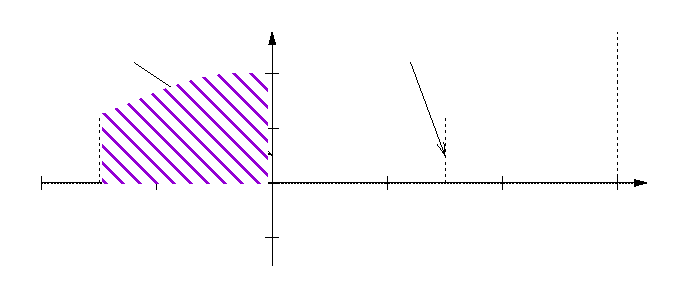
\includegraphics[width={316.80bp},height={129.50bp}]{figura_01_04}}%
    \gplfronttext
  \end{picture}%
\endgroup

    \caption{Demostración gráfica}\label{figura_04}
\end{figure}

\subsection*{Propiedad 4}
Si $b-a=T$:
\begin{equation}
    \int_{0}^{T}f(t)\,dt=\int_{a}^{b}f(t)\,dt
\label{propiedad4}
\end{equation}

\underline{Prueba}:

\begin{equation*}
\begin{split}
    \int_{a}^{b}f(t)\,dt
        &=\int_{a}^{a+T}f(t)\,dt\\
        &=\int_{a}^{T}f(t)\,dt+\int_{T}^{a+T}f(t)\,dt\\
        &=\int_{a}^{T}f(t)\,dt+\int_{T-T}^{a+T-T}f(t)\,dt\\
        &=\int_{a}^{T}f(t)\,dt+\int_{0}^{a}f(t)\,dt\\
        &=\int_{0}^{T}f(t)\,dt
\end{split}
\end{equation*}

Puede verse gráficamente en la \textbf{Figura~\ref{figura_05}}.
\begin{figure}[H]
    \centering
    % GNUPLOT: LaTeX picture with Postscript
\begingroup
  \makeatletter
  \providecommand\color[2][]{%
    \GenericError{(gnuplot) \space\space\space\@spaces}{%
      Package color not loaded in conjunction with
      terminal option `colourtext'%
    }{See the gnuplot documentation for explanation.%
    }{Either use 'blacktext' in gnuplot or load the package
      color.sty in LaTeX.}%
    \renewcommand\color[2][]{}%
  }%
  \providecommand\includegraphics[2][]{%
    \GenericError{(gnuplot) \space\space\space\@spaces}{%
      Package graphicx or graphics not loaded%
    }{See the gnuplot documentation for explanation.%
    }{The gnuplot epslatex terminal needs graphicx.sty or graphics.sty.}%
    \renewcommand\includegraphics[2][]{}%
  }%
  \providecommand\rotatebox[2]{#2}%
  \@ifundefined{ifGPcolor}{%
    \newif\ifGPcolor
    \GPcolorfalse
  }{}%
  \@ifundefined{ifGPblacktext}{%
    \newif\ifGPblacktext
    \GPblacktexttrue
  }{}%
  % define a \g@addto@macro without @ in the name:
  \let\gplgaddtomacro\g@addto@macro
  % define empty templates for all commands taking text:
  \gdef\gplbacktext{}%
  \gdef\gplfronttext{}%
  \makeatother
  \ifGPblacktext
    % no textcolor at all
    \def\colorrgb#1{}%
    \def\colorgray#1{}%
  \else
    % gray or color?
    \ifGPcolor
      \def\colorrgb#1{\color[rgb]{#1}}%
      \def\colorgray#1{\color[gray]{#1}}%
      \expandafter\def\csname LTw\endcsname{\color{white}}%
      \expandafter\def\csname LTb\endcsname{\color{black}}%
      \expandafter\def\csname LTa\endcsname{\color{black}}%
      \expandafter\def\csname LT0\endcsname{\color[rgb]{1,0,0}}%
      \expandafter\def\csname LT1\endcsname{\color[rgb]{0,1,0}}%
      \expandafter\def\csname LT2\endcsname{\color[rgb]{0,0,1}}%
      \expandafter\def\csname LT3\endcsname{\color[rgb]{1,0,1}}%
      \expandafter\def\csname LT4\endcsname{\color[rgb]{0,1,1}}%
      \expandafter\def\csname LT5\endcsname{\color[rgb]{1,1,0}}%
      \expandafter\def\csname LT6\endcsname{\color[rgb]{0,0,0}}%
      \expandafter\def\csname LT7\endcsname{\color[rgb]{1,0.3,0}}%
      \expandafter\def\csname LT8\endcsname{\color[rgb]{0.5,0.5,0.5}}%
    \else
      % gray
      \def\colorrgb#1{\color{black}}%
      \def\colorgray#1{\color[gray]{#1}}%
      \expandafter\def\csname LTw\endcsname{\color{white}}%
      \expandafter\def\csname LTb\endcsname{\color{black}}%
      \expandafter\def\csname LTa\endcsname{\color{black}}%
      \expandafter\def\csname LT0\endcsname{\color{black}}%
      \expandafter\def\csname LT1\endcsname{\color{black}}%
      \expandafter\def\csname LT2\endcsname{\color{black}}%
      \expandafter\def\csname LT3\endcsname{\color{black}}%
      \expandafter\def\csname LT4\endcsname{\color{black}}%
      \expandafter\def\csname LT5\endcsname{\color{black}}%
      \expandafter\def\csname LT6\endcsname{\color{black}}%
      \expandafter\def\csname LT7\endcsname{\color{black}}%
      \expandafter\def\csname LT8\endcsname{\color{black}}%
    \fi
  \fi
    \setlength{\unitlength}{0.0500bp}%
    \ifx\gptboxheight\undefined%
      \newlength{\gptboxheight}%
      \newlength{\gptboxwidth}%
      \newsavebox{\gptboxtext}%
    \fi%
    \setlength{\fboxrule}{0.5pt}%
    \setlength{\fboxsep}{1pt}%
    \definecolor{tbcol}{rgb}{1,1,1}%
\begin{picture}(6336.00,2590.00)%
    \gplgaddtomacro\gplbacktext{%
      \csname LTb\endcsname%%
      \put(1233,416){\makebox(0,0)[r]{\strut{}}}%
      \put(1233,863){\makebox(0,0)[r]{\strut{}}}%
      \put(1233,1311){\makebox(0,0)[r]{\strut{}}}%
      \put(1233,1758){\makebox(0,0)[r]{\strut{}}}%
      \put(1233,2205){\makebox(0,0)[r]{\strut{}}}%
      \put(603,640){\makebox(0,0){\strut{}}}%
      \put(1329,640){\makebox(0,0){\strut{}}}%
      \put(2055,640){\makebox(0,0){\strut{}}}%
      \put(2781,640){\makebox(0,0){\strut{}}}%
      \put(3506,640){\makebox(0,0){\strut{}}}%
      \put(4232,640){\makebox(0,0){\strut{}}}%
      \put(4958,640){\makebox(0,0){\strut{}}}%
      \put(5684,640){\makebox(0,0){\strut{}}}%
      \csname LTb\endcsname%%
      \put(6228,863){\makebox(0,0)[l]{\strut{}$t$}}%
      \put(1502,2429){\makebox(0,0)[l]{\strut{}$f(t)$}}%
      \put(2756,662){\makebox(0,0)[l]{\strut{}$a$}}%
      \put(3435,662){\makebox(0,0)[l]{\strut{}$T$}}%
      \put(4887,662){\makebox(0,0)[l]{\strut{}$b$}}%
      \put(1766,2026){\makebox(0,0)[l]{\strut{}$\int_{0}^{T} f(t) dt$}}%
      \put(3943,2295){\makebox(0,0)[l]{\strut{}$\int_{a}^{b} f(t) dt$}}%
      \put(3770,259){\makebox(0,0)[l]{\strut{}$T$}}%
    }%
    \gplgaddtomacro\gplfronttext{%
    }%
    \gplgaddtomacro\gplbacktext{%
      \csname LTb\endcsname%%
      \put(1233,416){\makebox(0,0)[r]{\strut{}}}%
      \put(1233,863){\makebox(0,0)[r]{\strut{}}}%
      \put(1233,1311){\makebox(0,0)[r]{\strut{}}}%
      \put(1233,1758){\makebox(0,0)[r]{\strut{}}}%
      \put(1233,2205){\makebox(0,0)[r]{\strut{}}}%
      \put(603,640){\makebox(0,0){\strut{}}}%
      \put(1329,640){\makebox(0,0){\strut{}}}%
      \put(2055,640){\makebox(0,0){\strut{}}}%
      \put(2781,640){\makebox(0,0){\strut{}}}%
      \put(3506,640){\makebox(0,0){\strut{}}}%
      \put(4232,640){\makebox(0,0){\strut{}}}%
      \put(4958,640){\makebox(0,0){\strut{}}}%
      \put(5684,640){\makebox(0,0){\strut{}}}%
      \csname LTb\endcsname%%
      \put(6228,863){\makebox(0,0)[l]{\strut{}$t$}}%
      \put(1502,2429){\makebox(0,0)[l]{\strut{}$f(t)$}}%
      \put(2756,662){\makebox(0,0)[l]{\strut{}$a$}}%
      \put(3435,662){\makebox(0,0)[l]{\strut{}$T$}}%
      \put(4887,662){\makebox(0,0)[l]{\strut{}$b$}}%
      \put(1766,2026){\makebox(0,0)[l]{\strut{}$\int_{0}^{T} f(t) dt$}}%
      \put(3943,2295){\makebox(0,0)[l]{\strut{}$\int_{a}^{b} f(t) dt$}}%
      \put(3770,259){\makebox(0,0)[l]{\strut{}$T$}}%
    }%
    \gplgaddtomacro\gplfronttext{%
    }%
    \gplgaddtomacro\gplbacktext{%
      \csname LTb\endcsname%%
      \put(1233,416){\makebox(0,0)[r]{\strut{}}}%
      \put(1233,863){\makebox(0,0)[r]{\strut{}}}%
      \put(1233,1311){\makebox(0,0)[r]{\strut{}}}%
      \put(1233,1758){\makebox(0,0)[r]{\strut{}}}%
      \put(1233,2205){\makebox(0,0)[r]{\strut{}}}%
      \put(603,640){\makebox(0,0){\strut{}}}%
      \put(1329,640){\makebox(0,0){\strut{}}}%
      \put(2055,640){\makebox(0,0){\strut{}}}%
      \put(2781,640){\makebox(0,0){\strut{}}}%
      \put(3506,640){\makebox(0,0){\strut{}}}%
      \put(4232,640){\makebox(0,0){\strut{}}}%
      \put(4958,640){\makebox(0,0){\strut{}}}%
      \put(5684,640){\makebox(0,0){\strut{}}}%
      \csname LTb\endcsname%%
      \put(6228,863){\makebox(0,0)[l]{\strut{}$t$}}%
      \put(1502,2429){\makebox(0,0)[l]{\strut{}$f(t)$}}%
      \put(2756,662){\makebox(0,0)[l]{\strut{}$a$}}%
      \put(3435,662){\makebox(0,0)[l]{\strut{}$T$}}%
      \put(4887,662){\makebox(0,0)[l]{\strut{}$b$}}%
      \put(1766,2026){\makebox(0,0)[l]{\strut{}$\int_{0}^{T} f(t) dt$}}%
      \put(3943,2295){\makebox(0,0)[l]{\strut{}$\int_{a}^{b} f(t) dt$}}%
      \put(3770,259){\makebox(0,0)[l]{\strut{}$T$}}%
    }%
    \gplgaddtomacro\gplfronttext{%
    }%
    \gplgaddtomacro\gplbacktext{%
      \csname LTb\endcsname%%
      \put(1233,416){\makebox(0,0)[r]{\strut{}}}%
      \put(1233,863){\makebox(0,0)[r]{\strut{}}}%
      \put(1233,1311){\makebox(0,0)[r]{\strut{}}}%
      \put(1233,1758){\makebox(0,0)[r]{\strut{}}}%
      \put(1233,2205){\makebox(0,0)[r]{\strut{}}}%
      \put(603,640){\makebox(0,0){\strut{}}}%
      \put(1329,640){\makebox(0,0){\strut{}}}%
      \put(2055,640){\makebox(0,0){\strut{}}}%
      \put(2781,640){\makebox(0,0){\strut{}}}%
      \put(3506,640){\makebox(0,0){\strut{}}}%
      \put(4232,640){\makebox(0,0){\strut{}}}%
      \put(4958,640){\makebox(0,0){\strut{}}}%
      \put(5684,640){\makebox(0,0){\strut{}}}%
      \csname LTb\endcsname%%
      \put(6228,863){\makebox(0,0)[l]{\strut{}$t$}}%
      \put(1502,2429){\makebox(0,0)[l]{\strut{}$f(t)$}}%
      \put(2756,662){\makebox(0,0)[l]{\strut{}$a$}}%
      \put(3435,662){\makebox(0,0)[l]{\strut{}$T$}}%
      \put(4887,662){\makebox(0,0)[l]{\strut{}$b$}}%
      \put(1766,2026){\makebox(0,0)[l]{\strut{}$\int_{0}^{T} f(t) dt$}}%
      \put(3943,2295){\makebox(0,0)[l]{\strut{}$\int_{a}^{b} f(t) dt$}}%
      \put(3770,259){\makebox(0,0)[l]{\strut{}$T$}}%
    }%
    \gplgaddtomacro\gplfronttext{%
    }%
    \gplgaddtomacro\gplbacktext{%
      \csname LTb\endcsname%%
      \put(1233,416){\makebox(0,0)[r]{\strut{}}}%
      \put(1233,863){\makebox(0,0)[r]{\strut{}}}%
      \put(1233,1311){\makebox(0,0)[r]{\strut{}}}%
      \put(1233,1758){\makebox(0,0)[r]{\strut{}}}%
      \put(1233,2205){\makebox(0,0)[r]{\strut{}}}%
      \put(603,640){\makebox(0,0){\strut{}}}%
      \put(1329,640){\makebox(0,0){\strut{}}}%
      \put(2055,640){\makebox(0,0){\strut{}}}%
      \put(2781,640){\makebox(0,0){\strut{}}}%
      \put(3506,640){\makebox(0,0){\strut{}}}%
      \put(4232,640){\makebox(0,0){\strut{}}}%
      \put(4958,640){\makebox(0,0){\strut{}}}%
      \put(5684,640){\makebox(0,0){\strut{}}}%
      \csname LTb\endcsname%%
      \put(6228,863){\makebox(0,0)[l]{\strut{}$t$}}%
      \put(1502,2429){\makebox(0,0)[l]{\strut{}$f(t)$}}%
      \put(2756,662){\makebox(0,0)[l]{\strut{}$a$}}%
      \put(3435,662){\makebox(0,0)[l]{\strut{}$T$}}%
      \put(4887,662){\makebox(0,0)[l]{\strut{}$b$}}%
      \put(1766,2026){\makebox(0,0)[l]{\strut{}$\int_{0}^{T} f(t) dt$}}%
      \put(3943,2295){\makebox(0,0)[l]{\strut{}$\int_{a}^{b} f(t) dt$}}%
      \put(3770,259){\makebox(0,0)[l]{\strut{}$T$}}%
    }%
    \gplgaddtomacro\gplfronttext{%
    }%
    \gplgaddtomacro\gplbacktext{%
      \csname LTb\endcsname%%
      \put(1233,416){\makebox(0,0)[r]{\strut{}}}%
      \put(1233,863){\makebox(0,0)[r]{\strut{}}}%
      \put(1233,1311){\makebox(0,0)[r]{\strut{}}}%
      \put(1233,1758){\makebox(0,0)[r]{\strut{}}}%
      \put(1233,2205){\makebox(0,0)[r]{\strut{}}}%
      \put(603,640){\makebox(0,0){\strut{}}}%
      \put(1329,640){\makebox(0,0){\strut{}}}%
      \put(2055,640){\makebox(0,0){\strut{}}}%
      \put(2781,640){\makebox(0,0){\strut{}}}%
      \put(3506,640){\makebox(0,0){\strut{}}}%
      \put(4232,640){\makebox(0,0){\strut{}}}%
      \put(4958,640){\makebox(0,0){\strut{}}}%
      \put(5684,640){\makebox(0,0){\strut{}}}%
      \csname LTb\endcsname%%
      \put(6228,863){\makebox(0,0)[l]{\strut{}$t$}}%
      \put(1502,2429){\makebox(0,0)[l]{\strut{}$f(t)$}}%
      \put(2756,662){\makebox(0,0)[l]{\strut{}$a$}}%
      \put(3435,662){\makebox(0,0)[l]{\strut{}$T$}}%
      \put(4887,662){\makebox(0,0)[l]{\strut{}$b$}}%
      \put(1766,2026){\makebox(0,0)[l]{\strut{}$\int_{0}^{T} f(t) dt$}}%
      \put(3943,2295){\makebox(0,0)[l]{\strut{}$\int_{a}^{b} f(t) dt$}}%
      \put(3770,259){\makebox(0,0)[l]{\strut{}$T$}}%
    }%
    \gplgaddtomacro\gplfronttext{%
    }%
    \gplgaddtomacro\gplbacktext{%
      \csname LTb\endcsname%%
      \put(1233,416){\makebox(0,0)[r]{\strut{}}}%
      \put(1233,863){\makebox(0,0)[r]{\strut{}}}%
      \put(1233,1311){\makebox(0,0)[r]{\strut{}}}%
      \put(1233,1758){\makebox(0,0)[r]{\strut{}}}%
      \put(1233,2205){\makebox(0,0)[r]{\strut{}}}%
      \put(603,640){\makebox(0,0){\strut{}}}%
      \put(1329,640){\makebox(0,0){\strut{}}}%
      \put(2055,640){\makebox(0,0){\strut{}}}%
      \put(2781,640){\makebox(0,0){\strut{}}}%
      \put(3506,640){\makebox(0,0){\strut{}}}%
      \put(4232,640){\makebox(0,0){\strut{}}}%
      \put(4958,640){\makebox(0,0){\strut{}}}%
      \put(5684,640){\makebox(0,0){\strut{}}}%
      \csname LTb\endcsname%%
      \put(6228,863){\makebox(0,0)[l]{\strut{}$t$}}%
      \put(1502,2429){\makebox(0,0)[l]{\strut{}$f(t)$}}%
      \put(2756,662){\makebox(0,0)[l]{\strut{}$a$}}%
      \put(3435,662){\makebox(0,0)[l]{\strut{}$T$}}%
      \put(4887,662){\makebox(0,0)[l]{\strut{}$b$}}%
      \put(1766,2026){\makebox(0,0)[l]{\strut{}$\int_{0}^{T} f(t) dt$}}%
      \put(3943,2295){\makebox(0,0)[l]{\strut{}$\int_{a}^{b} f(t) dt$}}%
      \put(3770,259){\makebox(0,0)[l]{\strut{}$T$}}%
    }%
    \gplgaddtomacro\gplfronttext{%
    }%
    \gplbacktext
    \put(0,0){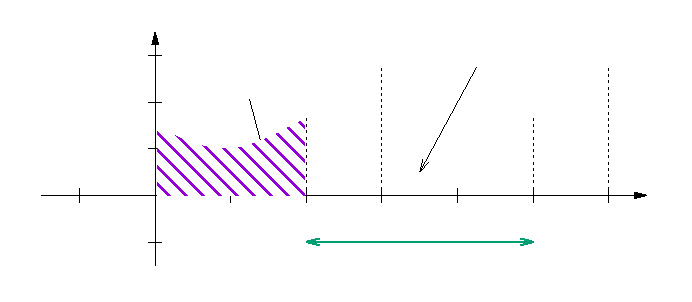
\includegraphics[width={316.80bp},height={129.50bp}]{figura_01_05}}%
    \gplfronttext
  \end{picture}%
\endgroup

    \caption{Demostración gráfica}\label{figura_05}
\end{figure}

\subsection{Funciones seno y coseno}
\begin{equation*}
    f(t)=A\,\sen(\omega_0\,t)
\end{equation*}
\begin{equation*}
    f(t)=A\,\cos(\omega_0\,t)
\end{equation*}

Donde:\\
\indent\indent$A$: Amplitud.\\
\indent\indent$\omega_0$: Frecuencia angular.\\
\indent\indent$T=2\pi/\omega_0$: Periodo.\\

\textbf{Ejemplo}: Hallar el periodo de la siguiente función:
\begin{equation*}
    f(t)=\sen(4t)+\sen(3t/2)+\sen(10t)
\end{equation*}

El periodo buscado debe contener un numero entero de veces a los 3 periodos
hallados:
\begin{equation*}
    T=\begin{cases}
        a\,T_1;&\,a\in\mathbb{N}\\
        b\,T_2;&\,b\in\mathbb{N}\\
        c\,T_3;&\,c\in\mathbb{N}\\
    \end{cases}
\end{equation*}
\begin{equation*}
    a\,T_1=b\,T_2=c\,T_3
\end{equation*}
\begin{equation*}
    a\,\frac{2\pi}{4}=b\,\frac{2\pi}{3/2}=c\,\frac{2\pi}{10}
\end{equation*}
\begin{equation*}
    a\,\frac{\pi}{2}=b\,\frac{4\pi}{3}=c\,\frac{\pi}{5};x30
\end{equation*}
\begin{equation*}
    15a=40b=6c
\end{equation*}
\begin{equation*}
    M.C.M.(15,40,6)=120
\end{equation*}
\begin{equation*}
\left.\begin{aligned}
    120=15a\rightarrow\,a=8\\
    120=40b\rightarrow\,b=3\\
    120=6c\rightarrow\,c=20\\
\end{aligned}\right\}=T=8\left(\frac{\pi}{2}\right)=4\pi
\end{equation*}

Puede verse gráficamente en la \textbf{Figura~\ref{figura_06}}.
\begin{figure}[H]
    \centering
    % GNUPLOT: LaTeX picture with Postscript
\begingroup
  \makeatletter
  \providecommand\color[2][]{%
    \GenericError{(gnuplot) \space\space\space\@spaces}{%
      Package color not loaded in conjunction with
      terminal option `colourtext'%
    }{See the gnuplot documentation for explanation.%
    }{Either use 'blacktext' in gnuplot or load the package
      color.sty in LaTeX.}%
    \renewcommand\color[2][]{}%
  }%
  \providecommand\includegraphics[2][]{%
    \GenericError{(gnuplot) \space\space\space\@spaces}{%
      Package graphicx or graphics not loaded%
    }{See the gnuplot documentation for explanation.%
    }{The gnuplot epslatex terminal needs graphicx.sty or graphics.sty.}%
    \renewcommand\includegraphics[2][]{}%
  }%
  \providecommand\rotatebox[2]{#2}%
  \@ifundefined{ifGPcolor}{%
    \newif\ifGPcolor
    \GPcolorfalse
  }{}%
  \@ifundefined{ifGPblacktext}{%
    \newif\ifGPblacktext
    \GPblacktexttrue
  }{}%
  % define a \g@addto@macro without @ in the name:
  \let\gplgaddtomacro\g@addto@macro
  % define empty templates for all commands taking text:
  \gdef\gplbacktext{}%
  \gdef\gplfronttext{}%
  \makeatother
  \ifGPblacktext
    % no textcolor at all
    \def\colorrgb#1{}%
    \def\colorgray#1{}%
  \else
    % gray or color?
    \ifGPcolor
      \def\colorrgb#1{\color[rgb]{#1}}%
      \def\colorgray#1{\color[gray]{#1}}%
      \expandafter\def\csname LTw\endcsname{\color{white}}%
      \expandafter\def\csname LTb\endcsname{\color{black}}%
      \expandafter\def\csname LTa\endcsname{\color{black}}%
      \expandafter\def\csname LT0\endcsname{\color[rgb]{1,0,0}}%
      \expandafter\def\csname LT1\endcsname{\color[rgb]{0,1,0}}%
      \expandafter\def\csname LT2\endcsname{\color[rgb]{0,0,1}}%
      \expandafter\def\csname LT3\endcsname{\color[rgb]{1,0,1}}%
      \expandafter\def\csname LT4\endcsname{\color[rgb]{0,1,1}}%
      \expandafter\def\csname LT5\endcsname{\color[rgb]{1,1,0}}%
      \expandafter\def\csname LT6\endcsname{\color[rgb]{0,0,0}}%
      \expandafter\def\csname LT7\endcsname{\color[rgb]{1,0.3,0}}%
      \expandafter\def\csname LT8\endcsname{\color[rgb]{0.5,0.5,0.5}}%
    \else
      % gray
      \def\colorrgb#1{\color{black}}%
      \def\colorgray#1{\color[gray]{#1}}%
      \expandafter\def\csname LTw\endcsname{\color{white}}%
      \expandafter\def\csname LTb\endcsname{\color{black}}%
      \expandafter\def\csname LTa\endcsname{\color{black}}%
      \expandafter\def\csname LT0\endcsname{\color{black}}%
      \expandafter\def\csname LT1\endcsname{\color{black}}%
      \expandafter\def\csname LT2\endcsname{\color{black}}%
      \expandafter\def\csname LT3\endcsname{\color{black}}%
      \expandafter\def\csname LT4\endcsname{\color{black}}%
      \expandafter\def\csname LT5\endcsname{\color{black}}%
      \expandafter\def\csname LT6\endcsname{\color{black}}%
      \expandafter\def\csname LT7\endcsname{\color{black}}%
      \expandafter\def\csname LT8\endcsname{\color{black}}%
    \fi
  \fi
    \setlength{\unitlength}{0.0500bp}%
    \ifx\gptboxheight\undefined%
      \newlength{\gptboxheight}%
      \newlength{\gptboxwidth}%
      \newsavebox{\gptboxtext}%
    \fi%
    \setlength{\fboxrule}{0.5pt}%
    \setlength{\fboxsep}{1pt}%
    \definecolor{tbcol}{rgb}{1,1,1}%
\begin{picture}(6336.00,1872.00)%
    \gplgaddtomacro\gplbacktext{%
      \csname LTb\endcsname%%
      \put(144,276){\makebox(0,0)[r]{\strut{}}}%
      \put(144,445){\makebox(0,0)[r]{\strut{}}}%
      \put(144,614){\makebox(0,0)[r]{\strut{}}}%
      \put(144,783){\makebox(0,0)[r]{\strut{}}}%
      \put(144,952){\makebox(0,0)[r]{\strut{}}}%
      \put(144,1120){\makebox(0,0)[r]{\strut{}}}%
      \put(144,1289){\makebox(0,0)[r]{\strut{}}}%
      \put(144,1458){\makebox(0,0)[r]{\strut{}}}%
      \put(144,1627){\makebox(0,0)[r]{\strut{}}}%
      \put(240,560){\makebox(0,0){\strut{}}}%
      \put(1606,560){\makebox(0,0){\strut{}}}%
      \put(2973,560){\makebox(0,0){\strut{}}}%
      \put(4339,560){\makebox(0,0){\strut{}}}%
      \put(5705,560){\makebox(0,0){\strut{}}}%
      \csname LTb\endcsname%%
      \put(6184,783){\makebox(0,0)[l]{\strut{}$t$}}%
      \put(392,1711){\makebox(0,0)[l]{\strut{}$f(t)$}}%
      \put(1541,656){\makebox(0,0)[l]{\strut{}$ \pi$}}%
      \put(2907,656){\makebox(0,0)[l]{\strut{}$2\pi$}}%
      \put(4274,656){\makebox(0,0)[l]{\strut{}$3\pi$}}%
      \put(5640,656){\makebox(0,0)[l]{\strut{}$4\pi$}}%
      \put(1606,1593){\makebox(0,0)[l]{\strut{}$f(t)=\sen(4t)+\sen(\frac{3}{2}t)+\sen(10t)\,dt$}}%
    }%
    \gplgaddtomacro\gplfronttext{%
    }%
    \gplbacktext
    \put(0,0){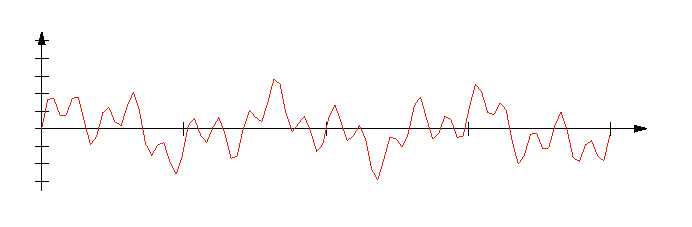
\includegraphics[width={316.80bp},height={93.60bp}]{figura_01_06}}%
    \gplfronttext
  \end{picture}%
\endgroup

    \caption{Periodo de la función}\label{figura_06}
\end{figure}

\subsection{Propiedades ortogonales del seno y el coseno}
\subsection*{Propiedad 1}
\begin{equation}
    \int_{0}^{T}\sen(n\omega_0\,t)\,dt=0\quad\,n\in\mathbb{Z}
\end{equation}

\underline{Prueba}:

\begin{equation*}
\begin{split}
    \int_{0}^{T}\sen(n\omega_0\,t)\,dt
        &=-\frac{\cos(n\omega_0\,t)}{n\omega_0}\Biggr|_{0}^{T}\\
        &=-\frac{\cos(n\omega_0\,T)}{n\omega_0}+\frac{\cos(0)}{n\omega_0}\\
        &=-\frac{\cos(n\,2\pi)}{n\omega_0}+\frac{\cos(0)}{n\omega_0}\\
        &=-\frac{1}{n\omega_0}+\frac{1}{n\omega_0}\\
        &=0\\
\end{split}
\end{equation*}
\begin{equation}
    \int_{0}^{T}\cos(n\omega_0\,t)\,dt=0\quad\,n\in\mathbb{Z}
\end{equation}

\underline{Prueba}:

\begin{equation*}
\begin{split}
    \int_{0}^{T}\cos(n\omega_0\,t)\,dt
        &=\frac{\sen(n\omega_0\,t)}{n\omega_0}\Biggr|_{0}^{T}\\
        &=\frac{\sen(n\omega_0\,T)}{n\omega_0}-\frac{\sen(0)}{n\omega_0}\\
        &=\frac{\sen(n\,2\pi)}{n\omega_0}-\frac{\sen(0)}{n\omega_0}\\
        &=\frac{0}{n\omega_0}-\frac{0}{n\omega_0}\\
        &=0\\
\end{split}
\end{equation*}

\subsection*{Propiedad 2}
\begin{equation}
    \int_{0}^{T}\sen(m\omega_0\,t)\sen(n\omega_0\,t)\,dt=0
    \quad\,m,n\,\in\mathbb{Z}\quad\,m\neq\,n
\end{equation}

\underline{Prueba}:

\begin{equation*}
\begin{split}
    \int_{0}^{T}\sen(m\omega_0\,t)\sen(n\omega_0\,t)\,dt
        &=\int_{0}^{T}\frac{1}{2}(\cos((m-n)\omega_0\,t)-
          \cos((m+n)\omega_0\,t))dt\\
        &=\frac{1}{2}\left(\int_{0}^{T}\cos((m-n)\omega_0\,t)dt-
          \int_{0}^{T}\cos((m+n)\omega_0\,t)dt\right)\\
        &=\frac{1}{2}(0-0)\\
        &=0\\
\end{split}
\end{equation*}
\begin{equation}
    \int_{0}^{T}\cos(m\omega_0\,t)\cos(n\omega_0\,t)\,dt=0
    \quad\,m,n\,\in\mathbb{Z}\quad\,m\neq\,n
\end{equation}

\underline{Prueba}:

\begin{equation*}
\begin{split}
    \int_{0}^{T}\cos(m\omega_0\,t)\cos(n\omega_0\,t)\,dt
        &=\int_{0}^{T}\frac{1}{2}(\cos((m-n)\omega_0\,t)+
          \cos((m+n)\omega_0\,t))dt\\
        &=\frac{1}{2}\left(\int_{0}^{T}\cos((m-n)\omega_0\,t)dt+
          \int_{0}^{T}\cos((m+n)\omega_0\,t)dt\right)\\
        &=\frac{1}{2}(0+0)\\
        &=0\\
\end{split}
\end{equation*}
\begin{equation}
    \int_{0}^{T}\sen(m\omega_0\,t)\cos(n\omega_0\,t)\,dt
    =0\quad\,m,n\,\in\mathbb{Z}
\end{equation}

\underline{Prueba}:

\begin{equation*}
\begin{split}
    \int_{0}^{T}\sen(m\omega_0\,t)\cos(n\omega_0\,t)\,dt
        &=\int_{0}^{T}\frac{1}{2}(\sen((m-n)\omega_0\,t)+
          \sen((m+n)\omega_0\,t))dt\\
        &=\frac{1}{2}\left(\int_{0}^{T}\sen((m-n)\omega_0\,t)dt+
          \int_{0}^{T}\cos((m+n)\omega_0\,t)dt\right)\\
        &=\frac{1}{2}(0+0)\\
        &=0\\
\end{split}
\end{equation*}

\subsection*{Propiedad 3}
\begin{equation}
    \int_{0}^{T}\sen^2(n\omega_0\,t)\,dt=\frac{T}{2}\quad\,n\,\in\mathbb{Z}
\end{equation}

\underline{Prueba}:

\begin{equation*}
\begin{split}
    \int_{0}^{T}\sen^2(n\omega_0\,t)\,dt
        &=\int_{0}^{T}\sen(n\omega_0\,t)\sen(n\omega_0\,t)dt\\
        &=\frac{1}{2}\left(\int_{0}^{T}\cos((n-n)\omega_0\,t)dt-
          \int_{0}^{T}\cos((n+n)\omega_0\,t)dt\right)\\
        &=\frac{1}{2}\left(\int_{0}^{T}\cos(0)dt-
          \int_{0}^{T}\cos((2n)\omega_0\,t)dt\right)\\
        &=\frac{1}{2}\left(\int_{0}^{T}dt-
          \int_{0}^{T}\cos(2n\omega_0\,t)dt\right)\\
        &=\frac{1}{2}(t\Biggr|_0^T-0)\\
        &=\frac{T}{2}\\
\end{split}
\end{equation*}
\begin{equation}
    \int_{0}^{T}\cos^2(n\omega_0\,t)\,dt=\frac{T}{2}\quad\,n\,\in\mathbb{Z}
\end{equation}

\underline{Prueba}:

\begin{equation*}
\begin{split}
    \int_{0}^{T}\cos^2(n\omega_0\,t)\,dt
        &=\int_{0}^{T}\cos(n\omega_0\,t)\cos(n\omega_0\,t)dt\\
        &=\frac{1}{2}\left(\int_{0}^{T}\cos((n-n)\omega_0\,t)dt+
          \int_{0}^{T}\cos((n+n)\omega_0\,t)dt\right)\\
        &=\frac{1}{2}\left(\int_{0}^{T}\cos(0)dt+
          \int_{0}^{T}\cos((2n)\omega_0\,t)dt\right)\\
        &=\frac{1}{2}\left(\int_{0}^{T}dt+
          \int_{0}^{T}\cos(2n\omega_0\,t)dt\right)\\
        &=\frac{1}{2}(t\Biggr|_0^T+0)\\
        &=\frac{T}{2}\\
\end{split}
\end{equation*}

\section{Series de \emph{Fourier}}
Una función periódica que cumple ciertas condiciones puede desarrollarse
mediante la serie:
\begin{equation}
    f(t)=\frac{a_0}{2}+
    \sum_{n=1}^{\infty}[a_n\cos(n\omega_0\,t)+b_n\sen(n\omega_0\,t)]
\end{equation}

Donde:\\
\indent\indent$\omega_0=2\pi/T$: Frecuencia angular de $f(t)$.\\
\indent\indent$T$: Periodo de $f(t)$.\\
\indent\indent$a_0;a_n;b_n$: Coeficientes de \emph{Fourier}.\\
\indent\indent$a_0/2$: Termino constante.\\
\indent\indent$a_n\cos(n\omega_0\,t);b_n\sen(n\omega_0\,t)$: Armónicos, términos
seno y coseno con frecuencias angulares múltiples de $\omega_0$\\

\indent\indent$a_1\cos(\omega_0\,t)+b_1\sen(\omega_0\,t)$: Primer armónico.\\
\indent\indent$a_2\cos(2\omega_0\,t)+b_2\sen(2\omega_0\,t)$: Segundo armónico.\\
\indent\indent$a_3\cos(3\omega_0\,t)+b_3\sen(2\omega_0\,t)$: Tercer armónico.\\

\subsection{Condiciones de \emph{Dirichlet}}
Para que una función periódica $f(t)=f(t+nT);\,n\in\mathbb{Z}$, se desarrolle
como una serie de \emph{Fourier} debe cumplir:

\begin{itemize}
\item $f(t)$ debe ser continua por tramos en 1 periodo.
    \begin{figure}[H]
        \centering
        % GNUPLOT: LaTeX picture with Postscript
\begingroup
  \makeatletter
  \providecommand\color[2][]{%
    \GenericError{(gnuplot) \space\space\space\@spaces}{%
      Package color not loaded in conjunction with
      terminal option `colourtext'%
    }{See the gnuplot documentation for explanation.%
    }{Either use 'blacktext' in gnuplot or load the package
      color.sty in LaTeX.}%
    \renewcommand\color[2][]{}%
  }%
  \providecommand\includegraphics[2][]{%
    \GenericError{(gnuplot) \space\space\space\@spaces}{%
      Package graphicx or graphics not loaded%
    }{See the gnuplot documentation for explanation.%
    }{The gnuplot epslatex terminal needs graphicx.sty or graphics.sty.}%
    \renewcommand\includegraphics[2][]{}%
  }%
  \providecommand\rotatebox[2]{#2}%
  \@ifundefined{ifGPcolor}{%
    \newif\ifGPcolor
    \GPcolorfalse
  }{}%
  \@ifundefined{ifGPblacktext}{%
    \newif\ifGPblacktext
    \GPblacktexttrue
  }{}%
  % define a \g@addto@macro without @ in the name:
  \let\gplgaddtomacro\g@addto@macro
  % define empty templates for all commands taking text:
  \gdef\gplbacktext{}%
  \gdef\gplfronttext{}%
  \makeatother
  \ifGPblacktext
    % no textcolor at all
    \def\colorrgb#1{}%
    \def\colorgray#1{}%
  \else
    % gray or color?
    \ifGPcolor
      \def\colorrgb#1{\color[rgb]{#1}}%
      \def\colorgray#1{\color[gray]{#1}}%
      \expandafter\def\csname LTw\endcsname{\color{white}}%
      \expandafter\def\csname LTb\endcsname{\color{black}}%
      \expandafter\def\csname LTa\endcsname{\color{black}}%
      \expandafter\def\csname LT0\endcsname{\color[rgb]{1,0,0}}%
      \expandafter\def\csname LT1\endcsname{\color[rgb]{0,1,0}}%
      \expandafter\def\csname LT2\endcsname{\color[rgb]{0,0,1}}%
      \expandafter\def\csname LT3\endcsname{\color[rgb]{1,0,1}}%
      \expandafter\def\csname LT4\endcsname{\color[rgb]{0,1,1}}%
      \expandafter\def\csname LT5\endcsname{\color[rgb]{1,1,0}}%
      \expandafter\def\csname LT6\endcsname{\color[rgb]{0,0,0}}%
      \expandafter\def\csname LT7\endcsname{\color[rgb]{1,0.3,0}}%
      \expandafter\def\csname LT8\endcsname{\color[rgb]{0.5,0.5,0.5}}%
    \else
      % gray
      \def\colorrgb#1{\color{black}}%
      \def\colorgray#1{\color[gray]{#1}}%
      \expandafter\def\csname LTw\endcsname{\color{white}}%
      \expandafter\def\csname LTb\endcsname{\color{black}}%
      \expandafter\def\csname LTa\endcsname{\color{black}}%
      \expandafter\def\csname LT0\endcsname{\color{black}}%
      \expandafter\def\csname LT1\endcsname{\color{black}}%
      \expandafter\def\csname LT2\endcsname{\color{black}}%
      \expandafter\def\csname LT3\endcsname{\color{black}}%
      \expandafter\def\csname LT4\endcsname{\color{black}}%
      \expandafter\def\csname LT5\endcsname{\color{black}}%
      \expandafter\def\csname LT6\endcsname{\color{black}}%
      \expandafter\def\csname LT7\endcsname{\color{black}}%
      \expandafter\def\csname LT8\endcsname{\color{black}}%
    \fi
  \fi
    \setlength{\unitlength}{0.0500bp}%
    \ifx\gptboxheight\undefined%
      \newlength{\gptboxheight}%
      \newlength{\gptboxwidth}%
      \newsavebox{\gptboxtext}%
    \fi%
    \setlength{\fboxrule}{0.5pt}%
    \setlength{\fboxsep}{1pt}%
    \definecolor{tbcol}{rgb}{1,1,1}%
\begin{picture}(6336.00,2590.00)%
    \gplgaddtomacro\gplbacktext{%
      \csname LTb\endcsname%%
      \put(628,352){\makebox(0,0)[r]{\strut{}}}%
      \put(628,671){\makebox(0,0)[r]{\strut{}}}%
      \put(628,991){\makebox(0,0)[r]{\strut{}}}%
      \put(628,1311){\makebox(0,0)[r]{\strut{}}}%
      \put(628,1630){\makebox(0,0)[r]{\strut{}}}%
      \put(628,1950){\makebox(0,0)[r]{\strut{}}}%
      \put(628,2269){\makebox(0,0)[r]{\strut{}}}%
      \put(724,1088){\makebox(0,0){\strut{}}}%
      \put(1692,1088){\makebox(0,0){\strut{}}}%
      \put(2660,1088){\makebox(0,0){\strut{}}}%
      \put(3627,1088){\makebox(0,0){\strut{}}}%
      \put(4595,1088){\makebox(0,0){\strut{}}}%
      \put(5563,1088){\makebox(0,0){\strut{}}}%
      \csname LTb\endcsname%%
      \put(6289,1311){\makebox(0,0)[l]{\strut{}$t$}}%
      \put(579,2589){\makebox(0,0)[l]{\strut{}$f(t)$}}%
      \put(2611,1071){\makebox(0,0)[l]{\strut{}$t_1$}}%
      \put(3579,1071){\makebox(0,0)[l]{\strut{}$t_2$}}%
      \put(5515,1071){\makebox(0,0)[l]{\strut{}$T$}}%
      \put(3627,2333){\makebox(0,0)[l]{\strut{}discontinuidad}}%
      \put(4111,2014){\makebox(0,0)[l]{\strut{}extremo relativo}}%
    }%
    \gplgaddtomacro\gplfronttext{%
    }%
    \gplgaddtomacro\gplbacktext{%
      \csname LTb\endcsname%%
      \put(628,352){\makebox(0,0)[r]{\strut{}}}%
      \put(628,671){\makebox(0,0)[r]{\strut{}}}%
      \put(628,991){\makebox(0,0)[r]{\strut{}}}%
      \put(628,1311){\makebox(0,0)[r]{\strut{}}}%
      \put(628,1630){\makebox(0,0)[r]{\strut{}}}%
      \put(628,1950){\makebox(0,0)[r]{\strut{}}}%
      \put(628,2269){\makebox(0,0)[r]{\strut{}}}%
      \put(724,1088){\makebox(0,0){\strut{}}}%
      \put(1692,1088){\makebox(0,0){\strut{}}}%
      \put(2660,1088){\makebox(0,0){\strut{}}}%
      \put(3627,1088){\makebox(0,0){\strut{}}}%
      \put(4595,1088){\makebox(0,0){\strut{}}}%
      \put(5563,1088){\makebox(0,0){\strut{}}}%
      \csname LTb\endcsname%%
      \put(6289,1311){\makebox(0,0)[l]{\strut{}$t$}}%
      \put(579,2589){\makebox(0,0)[l]{\strut{}$f(t)$}}%
      \put(2611,1071){\makebox(0,0)[l]{\strut{}$t_1$}}%
      \put(3579,1071){\makebox(0,0)[l]{\strut{}$t_2$}}%
      \put(5515,1071){\makebox(0,0)[l]{\strut{}$T$}}%
      \put(3627,2333){\makebox(0,0)[l]{\strut{}discontinuidad}}%
      \put(4111,2014){\makebox(0,0)[l]{\strut{}extremo relativo}}%
    }%
    \gplgaddtomacro\gplfronttext{%
    }%
    \gplgaddtomacro\gplbacktext{%
      \csname LTb\endcsname%%
      \put(628,352){\makebox(0,0)[r]{\strut{}}}%
      \put(628,671){\makebox(0,0)[r]{\strut{}}}%
      \put(628,991){\makebox(0,0)[r]{\strut{}}}%
      \put(628,1311){\makebox(0,0)[r]{\strut{}}}%
      \put(628,1630){\makebox(0,0)[r]{\strut{}}}%
      \put(628,1950){\makebox(0,0)[r]{\strut{}}}%
      \put(628,2269){\makebox(0,0)[r]{\strut{}}}%
      \put(724,1088){\makebox(0,0){\strut{}}}%
      \put(1692,1088){\makebox(0,0){\strut{}}}%
      \put(2660,1088){\makebox(0,0){\strut{}}}%
      \put(3627,1088){\makebox(0,0){\strut{}}}%
      \put(4595,1088){\makebox(0,0){\strut{}}}%
      \put(5563,1088){\makebox(0,0){\strut{}}}%
      \csname LTb\endcsname%%
      \put(6289,1311){\makebox(0,0)[l]{\strut{}$t$}}%
      \put(579,2589){\makebox(0,0)[l]{\strut{}$f(t)$}}%
      \put(2611,1071){\makebox(0,0)[l]{\strut{}$t_1$}}%
      \put(3579,1071){\makebox(0,0)[l]{\strut{}$t_2$}}%
      \put(5515,1071){\makebox(0,0)[l]{\strut{}$T$}}%
      \put(3627,2333){\makebox(0,0)[l]{\strut{}discontinuidad}}%
      \put(4111,2014){\makebox(0,0)[l]{\strut{}extremo relativo}}%
    }%
    \gplgaddtomacro\gplfronttext{%
    }%
    \gplbacktext
    \put(0,0){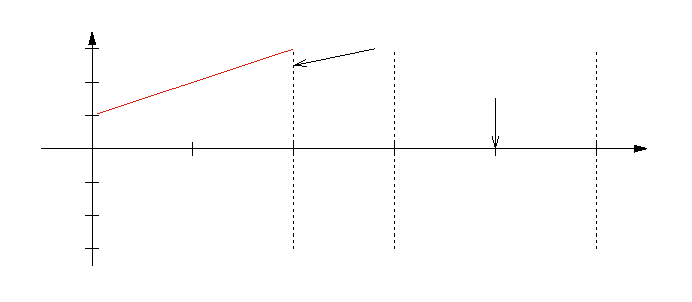
\includegraphics[width={316.80bp},height={129.50bp}]{figura_01_07}}%
    \gplfronttext
  \end{picture}%
\endgroup

    \end{figure}
    \begin{itemize}
    \item Debe existir un numero finito de discontinuidades (en 1 periodo).
    \item Debe existir un numero finito de extremos relativos (en 1 periodo).
    \end{itemize}
\item La integral $\int_0^T|f(t)|\,dt<\infty$ debe ser finita.
\end{itemize}

\textbf{Ejemplo}:
\begin{equation*}
    f(t)=\tan(t);\quad\,0<t<\pi;\quad\,T=\pi
\end{equation*}
\begin{figure}[H]
    \centering
    % GNUPLOT: LaTeX picture with Postscript
\begingroup
  \makeatletter
  \providecommand\color[2][]{%
    \GenericError{(gnuplot) \space\space\space\@spaces}{%
      Package color not loaded in conjunction with
      terminal option `colourtext'%
    }{See the gnuplot documentation for explanation.%
    }{Either use 'blacktext' in gnuplot or load the package
      color.sty in LaTeX.}%
    \renewcommand\color[2][]{}%
  }%
  \providecommand\includegraphics[2][]{%
    \GenericError{(gnuplot) \space\space\space\@spaces}{%
      Package graphicx or graphics not loaded%
    }{See the gnuplot documentation for explanation.%
    }{The gnuplot epslatex terminal needs graphicx.sty or graphics.sty.}%
    \renewcommand\includegraphics[2][]{}%
  }%
  \providecommand\rotatebox[2]{#2}%
  \@ifundefined{ifGPcolor}{%
    \newif\ifGPcolor
    \GPcolorfalse
  }{}%
  \@ifundefined{ifGPblacktext}{%
    \newif\ifGPblacktext
    \GPblacktexttrue
  }{}%
  % define a \g@addto@macro without @ in the name:
  \let\gplgaddtomacro\g@addto@macro
  % define empty templates for all commands taking text:
  \gdef\gplbacktext{}%
  \gdef\gplfronttext{}%
  \makeatother
  \ifGPblacktext
    % no textcolor at all
    \def\colorrgb#1{}%
    \def\colorgray#1{}%
  \else
    % gray or color?
    \ifGPcolor
      \def\colorrgb#1{\color[rgb]{#1}}%
      \def\colorgray#1{\color[gray]{#1}}%
      \expandafter\def\csname LTw\endcsname{\color{white}}%
      \expandafter\def\csname LTb\endcsname{\color{black}}%
      \expandafter\def\csname LTa\endcsname{\color{black}}%
      \expandafter\def\csname LT0\endcsname{\color[rgb]{1,0,0}}%
      \expandafter\def\csname LT1\endcsname{\color[rgb]{0,1,0}}%
      \expandafter\def\csname LT2\endcsname{\color[rgb]{0,0,1}}%
      \expandafter\def\csname LT3\endcsname{\color[rgb]{1,0,1}}%
      \expandafter\def\csname LT4\endcsname{\color[rgb]{0,1,1}}%
      \expandafter\def\csname LT5\endcsname{\color[rgb]{1,1,0}}%
      \expandafter\def\csname LT6\endcsname{\color[rgb]{0,0,0}}%
      \expandafter\def\csname LT7\endcsname{\color[rgb]{1,0.3,0}}%
      \expandafter\def\csname LT8\endcsname{\color[rgb]{0.5,0.5,0.5}}%
    \else
      % gray
      \def\colorrgb#1{\color{black}}%
      \def\colorgray#1{\color[gray]{#1}}%
      \expandafter\def\csname LTw\endcsname{\color{white}}%
      \expandafter\def\csname LTb\endcsname{\color{black}}%
      \expandafter\def\csname LTa\endcsname{\color{black}}%
      \expandafter\def\csname LT0\endcsname{\color{black}}%
      \expandafter\def\csname LT1\endcsname{\color{black}}%
      \expandafter\def\csname LT2\endcsname{\color{black}}%
      \expandafter\def\csname LT3\endcsname{\color{black}}%
      \expandafter\def\csname LT4\endcsname{\color{black}}%
      \expandafter\def\csname LT5\endcsname{\color{black}}%
      \expandafter\def\csname LT6\endcsname{\color{black}}%
      \expandafter\def\csname LT7\endcsname{\color{black}}%
      \expandafter\def\csname LT8\endcsname{\color{black}}%
    \fi
  \fi
    \setlength{\unitlength}{0.0500bp}%
    \ifx\gptboxheight\undefined%
      \newlength{\gptboxheight}%
      \newlength{\gptboxwidth}%
      \newsavebox{\gptboxtext}%
    \fi%
    \setlength{\fboxrule}{0.5pt}%
    \setlength{\fboxsep}{1pt}%
    \definecolor{tbcol}{rgb}{1,1,1}%
\begin{picture}(4320.00,4320.00)%
    \gplgaddtomacro\gplbacktext{%
      \csname LTb\endcsname%%
      \put(2040,192){\makebox(0,0)[r]{\strut{}}}%
      \put(2040,390){\makebox(0,0)[r]{\strut{}}}%
      \put(2040,589){\makebox(0,0)[r]{\strut{}}}%
      \put(2040,787){\makebox(0,0)[r]{\strut{}}}%
      \put(2040,985){\makebox(0,0)[r]{\strut{}}}%
      \put(2040,1184){\makebox(0,0)[r]{\strut{}}}%
      \put(2040,1382){\makebox(0,0)[r]{\strut{}}}%
      \put(2040,1580){\makebox(0,0)[r]{\strut{}}}%
      \put(2040,1779){\makebox(0,0)[r]{\strut{}}}%
      \put(2040,1977){\makebox(0,0)[r]{\strut{}}}%
      \put(2040,2176){\makebox(0,0)[r]{\strut{}}}%
      \put(2040,2374){\makebox(0,0)[r]{\strut{}}}%
      \put(2040,2572){\makebox(0,0)[r]{\strut{}}}%
      \put(2040,2771){\makebox(0,0)[r]{\strut{}}}%
      \put(2040,2969){\makebox(0,0)[r]{\strut{}}}%
      \put(2040,3167){\makebox(0,0)[r]{\strut{}}}%
      \put(2040,3366){\makebox(0,0)[r]{\strut{}}}%
      \put(2040,3564){\makebox(0,0)[r]{\strut{}}}%
      \put(2040,3762){\makebox(0,0)[r]{\strut{}}}%
      \put(2040,3961){\makebox(0,0)[r]{\strut{}}}%
      \put(2040,4159){\makebox(0,0)[r]{\strut{}}}%
      \put(511,1953){\makebox(0,0){\strut{}}}%
      \put(1052,1953){\makebox(0,0){\strut{}}}%
      \put(1594,1953){\makebox(0,0){\strut{}}}%
      \put(2136,1953){\makebox(0,0){\strut{}}}%
      \put(2677,1953){\makebox(0,0){\strut{}}}%
      \put(3219,1953){\makebox(0,0){\strut{}}}%
      \put(3760,1953){\makebox(0,0){\strut{}}}%
      \csname LTb\endcsname%%
      \put(4302,2176){\makebox(0,0)[l]{\strut{}$t$}}%
      \put(2015,4357){\makebox(0,0)[l]{\strut{}$f(t)$}}%
      \put(2574,1878){\makebox(0,0)[l]{\strut{}$\frac{\pi}{2}$}}%
      \put(3115,1878){\makebox(0,0)[l]{\strut{}$\pi$}}%
    }%
    \gplgaddtomacro\gplfronttext{%
    }%
    \gplbacktext
    \put(0,0){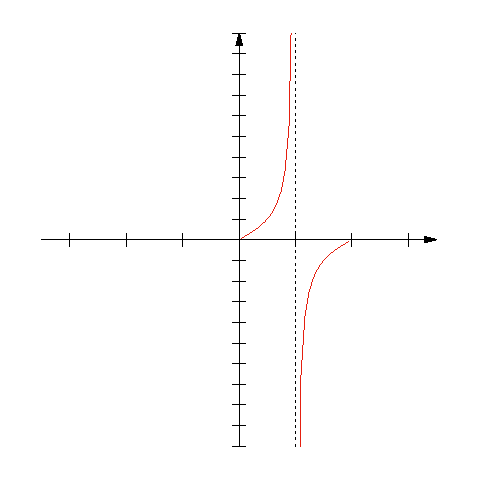
\includegraphics[width={216.00bp},height={216.00bp}]{figura_01_08}}%
    \gplfronttext
  \end{picture}%
\endgroup

\end{figure}
\begin{equation*}
    \int_0^\pi|\tan(t)|\,dt\rightarrow\infty
\end{equation*}
\begin{equation*}
    t=\frac{\pi}{2}:|\tan(t)|\rightarrow\infty
\end{equation*}
\\
\begin{equation*}
    \therefore\,\text{Esta función no tiene serie de \emph{Fourier}.}
\end{equation*}

\section{Evaluación de los coeficientes de \emph{Fourier}}
\begin{equation*}
    f(t)=\frac{a_0}{2}+
    \sum_{n=1}^{\infty}[a_n\cos(n\omega_0\,t)+b_n\sen(n\omega_0\,t)]
\end{equation*}

Integrando ambas partes:
\begin{equation*}
\begin{split}
    \int_{0}^{T}f(t)\,dt
        &=\int_{0}^{T}\frac{a_0}{2}\,dt+
          \sum_{n=1}^{\infty}\left[\int_{0}^{T}a_n\cos(n\omega_0\,t)\,dt+
          \int_{0}^{T}b_n\sen(n\omega_0\,t)\,dt\right]\\
        &=\frac{a_0}{2}t\Biggr|_{0}^{T}\\
        &=\frac{a_0}{2}T\\
\end{split}
\end{equation*}
\begin{equation}
    a_0=\frac{2}{T}\int_{0}^{T}f(t)\,dt
\end{equation}

Para calcular ``$a_n$'' multiplicamos por $\cos(m\omega_0\,t);m\in\mathbb{N}$ e
integramos en 1 periodo.
\begin{equation*}
\begin{split}
    \int_{0}^{T}f(t)\cos(m\omega_0\,t)\,dt
        &=\int_{0}^{T}\frac{a_0}{2}\cos(m\omega_0\,t)\,dt\\
        &+\sum_{n=1}^{\infty}\left[
          \int_{0}^{T}a_n\cos(n\omega_0\,t)\cos(m\omega_0\,t)\,dt+
          \int_{0}^{T}b_n\sen(n\omega_0\,t)\cos(m\omega_0\,t)\,dt\right]\\
        &=0+\sum_{n=1}^{\infty}\left[
          \int_{0}^{T}a_n\cos(n\omega_0\,t)\cos(m\omega_0\,t)\,dt+0\right]\\
\end{split}
\end{equation*}

Para $n\neq m$ todos los elementos de la sumatoria serán igual a $0$.
Por tanto:
\begin{equation*}
\begin{split}
    \int_{0}^{T}f(t)\cos(n\omega_0\,t)\,dt
        &=\int_{0}^{T}a_n\cos^2(n\omega_0\,t)\,dt\\
        &=a_n\frac{T}{2}\\
\end{split}
\end{equation*}
\begin{equation}
    a_n=\frac{2}{T}\int_{0}^{T}f(t)\cos(n\omega_0\,t)\,dt
\end{equation}

Para calcular ``$b_n$'' multiplicamos por $\sen(m\omega_0\,t);m\in\mathbb{N}$ e
integramos en 1 periodo.
\begin{equation*}
\begin{split}
    \int_{0}^{T}f(t)\sen(m\omega_0\,t)\,dt
        &=\int_{0}^{T}\frac{a_0}{2}\sen(m\omega_0\,t)\,dt\\
        &+\sum_{n=1}^{\infty}\left[
          \int_{0}^{T}a_n\cos(n\omega_0\,t)\sen(m\omega_0\,t)\,dt+
          \int_{0}^{T}b_n\sen(n\omega_0\,t)\sen(m\omega_0\,t)\,dt\right]\\
        &=0+\sum_{n=1}^{\infty}\left[
          0+\int_{0}^{T}b_n\sen(n\omega_0\,t)\sen(m\omega_0\,t)\,dt\right]\\
\end{split}
\end{equation*}

Para $n\neq\,m$ todos los elementos de la sumatoria serán igual a $0$.
Por tanto:
\begin{equation*}
\begin{split}
    \int_{0}^{T}f(t)\sen(n\omega_0\,t)\,dt
        &=\int_{0}^{T}b_n\sen^2(n\omega_0\,t)\,dt\\
        &=b_n\,\frac{T}{2}\\
\end{split}
\end{equation*}
\begin{equation}
    b_n=\frac{2}{T}\int_{0}^{T}f(t)\sen(n\omega_0\,t)\,dt
\end{equation}

\section{Formulas para las series de \emph{Fourier}}
\begin{equation*}
    \sen(\pi\,n)=0;\quad\,n\in\mathbb{N}
\end{equation*}
\begin{equation*}
    \cos(\pi\,n)={(-1)}^n;\quad\,n\in\mathbb{N}
\end{equation*}
\begin{equation*}
    \sen(2\pi\,n)=0;\quad\,n\in\mathbb{N}
\end{equation*}
\begin{equation*}
    \cos(2\pi\,n)=1;\quad\,n\in\mathbb{N}
\end{equation*}
\begin{equation*}
    \int\,\sen(at)\,dt=-\frac{\cos(at)}{a}
\end{equation*}
\begin{equation*}
    \int\,\cos(at)\,dt=\frac{\sen(at)}{a}
\end{equation*}
\begin{equation*}
    \int\,t\sen(at)\,dt=-\frac{t}{a}\cos(at)+\frac{1}{a^2}\sen(at)
\end{equation*}
\begin{equation*}
    \int\,t\cos(at)\,dt=\frac{t}{a}\sen(at)+\frac{1}{a^2}\cos(at)
\end{equation*}
\begin{equation*}
    \int\,{e}^{at}\,dt=\frac{1}{a}e^{at}
\end{equation*}
\begin{equation*}
    \int\,t\,{e}^{at}\,dt=\frac{t}{a}\,{e}^{at}-\frac{1}{a^2}{e}^{at}
\end{equation*}

